\section{Decentralized Swarm Coordination via Broadcast-as-Shared-State:
A Four-Layer Architecture with Empirical
Validation}\label{decentralized-swarm-coordination-via-broadcast-as-shared-state-a-four-layer-architecture-with-empirical-validation}

\subsection{Contents}\label{contents}

\begin{enumerate}
\def\labelenumi{\arabic{enumi}.}
\tightlist
\item
  \hyperref[1-introduction]{Introduction}
\item
  \hyperref[2-notation-and-the-substrate-primitive]{Notation and the
  substrate primitive}
\item
  \hyperref[3-layer-1-hierarchical-assignment]{Layer 1: Hierarchical
  assignment}
\item
  \hyperref[4-layer-2-local-recovery]{Layer 2: Local recovery}
\item
  \hyperref[5-layer-3-priority-allocation]{Layer 3: Priority allocation}
\item
  \hyperref[6-layer-4-localization]{Layer 4: Localization}
\item
  \hyperref[7-substrate-composition]{Substrate composition}
\item
  \hyperref[8-related-work]{Related work}
\item
  \hyperref[9-discussion]{Discussion}
\item
  \hyperref[10-future-work]{Future work}
\item
  \hyperref[11-reproducing]{Reproducing}
\end{enumerate}

Companion files: - \texttt{PROOFS.md} --- formal lemmas and theorems -
\texttt{figures/} --- generated plots - \texttt{swarm.mp4} --- rendered
four-phase demo - Source: \texttt{simulator.py}, \texttt{bench\_*.py},
\texttt{make\_figures.py}

\textbf{Code and data availability.} All source, simulator, benchmark
scripts, figures, and the rendered four-phase demo are archived at
Zenodo under DOI
\href{https://doi.org/10.5281/zenodo.20385946}{10.5281/zenodo.20385946}
and mirrored at the GitHub repository
\href{https://github.com/jmcentire/drone-swarm-coordination}{github.com/jmcentire/drone-swarm-coordination}.
The Zenodo deposition is the citable, version-pinned snapshot; the
GitHub repository tracks ongoing changes.

\subsection{Abstract}\label{abstract}

Prior work has addressed dynamic assignment via centralized incremental
algorithms (Toroslu \& Üçoluk 2007), hardware redundancy via intra-drone
shadow nodes (Kim \& Welch 1989, DRB framework), GPS-denied operation
via improved per-drone state estimation (Allan-variance fusion, RNN-EKF
replacement), and assignment stability via centralized hysteresis-aware
reinforcement learning. We present a unified architecture that addresses
these concerns through a single decentralized primitive in the
four-layer regime: broadcast-shared state with locally- deterministic
computation. The architecture's four mechanisms --- hierarchical
bisection assignment, local patch recovery, sub-manifold shadow
allocation, and confidence-thresholded fiducial selection --- share a
common substrate and are independently provable, with empirical
validation across N=10 to N=10,000. The v1.2 supplemental (§9.4)
characterizes the substrate's empirical envelope on three operational
mission classes (drift handling, online replanning, Bayesian search-
and-rescue) where degraded-comms regimes additionally require a
majority-vote aggregation primitive whose contribution is characterized
empirically rather than claimed as architectural novelty.

Headline empirical results: assignment within 1.4--3\% of the Hungarian
optimum (gap empirically fits \texttt{a\ +\ b/√N} better than
alternatives; rounding contribution provably O(1/√N),
projection-half-cut bound open); patch protocol produces exactly one
reassignment per death up to surplus capacity; tiered shadow allocation
reduces flight cost 66\% (pure key shadow vs uniform) when threats
correlate with priority; Layer 4's fiducial-selection plus cooperative
localization reduces formation error 4× vs sparse-GPS baseline (4cm vs
17cm) under per-drone Poisson GPS at 0.1/s. The substrate generalization
claim --- that one primitive suffices for four distinct coordination
patterns --- is empirically validated by the composition of all four
mechanisms in working simulations (\texttt{simulator.py} for Layers
1--3, \texttt{bench\_layer4.py} for Layer 4), with formal properties
established in a companion proofs document.

The v1.3 supplemental adds a bounded underwater feasibility track. It
does \textbf{not} claim that the full underwater mission protocol is
solved: earlier underwater mission-loop benches that used
centralized/oracle state are excluded from the evidentiary base. The
valid underwater results reported here are narrower: range-limited
detection-map gossip, acoustic link-budget and throughput accounting,
and vertical acoustic relay localization. These results establish
physically-grounded modeling targets and mechanisms for a future
per-drone adaptive underwater mission loop.

\subsection{1. Introduction}\label{introduction}

A swarm of N drones is given the task of forming a target shape M of N
positions. Three operational concerns stack:

\begin{enumerate}
\def\labelenumi{\arabic{enumi}.}
\tightlist
\item
  \textbf{Assignment}: which drone goes to which leaf of M?
\item
  \textbf{Recovery}: when a drone is lost mid-mission, which surplus
  drone takes over its leaf, and how does the rest of the swarm respond?
\item
  \textbf{Priority allocation}: when redundancy is finite, which leaves
  get the protection budget?
\end{enumerate}

A fourth concern --- \textbf{localization} --- applies to any swarm
operating under realistic sensor noise, where GPS may be intermittent
and drones must dead-reckon between fixes.

Existing approaches treat these as separate problems requiring separate
mechanisms. CAPT (Turpin et al.~2014) handles assignment via Hungarian
matching, requiring centralized computation; CBBA (Choi et al.~2009)
distributes the auction but requires multiple rounds of inter-agent
communication. Loss recovery in either approach requires re-running the
optimization, paying the full cost again. Priority allocation is
typically handled by hand-coded role assignments. Localization is a
separate filtering layer (EKF or particle filter) that uses GPS and IMU
data without participating in the swarm coordination.

This work observes that all four concerns admit decentralized solutions
on the same primitive: a shared broadcast medium where each agent
maintains its slot and reads everyone else's, with consensus arising
from determinism (same input + same algorithm = same output) rather than
message-passing protocols.

The architectural contribution is the \textbf{substrate}: a single
primitive that supports four cleanly separated mechanisms. The empirical
contribution is validation of each mechanism in isolation and in
composition, against baselines where applicable. The theoretical
contribution is a set of lemmas establishing determinism, bijectivity,
and patch optimality, with conjectured asymptotic bounds on the
optimality gap.

\subsection{2. Notation and the substrate
primitive}\label{notation-and-the-substrate-primitive}

Notation conventions follow \texttt{PROOFS.md}, which contains formal
statements and proofs of all results referenced in this section.

\textbf{Target manifold} M = \{m₁, \ldots, m\_N\} ⊂ ℝ³ is a set of N
target positions the swarm is to occupy. The \textbf{PCA tree} T(M) is
the binary tree obtained by recursive principal-axis splits: each
internal node v has a leaf set L\_v ⊆ M, a centroid c\_v = mean(L\_v),
and a split direction Π\_v (the dominant right-singular vector of L\_v -
c\_v); its children partition L\_v at the projection median.

\textbf{Drone set} D = \{d₁, \ldots, d\_n\} with positions p(d\_i) ∈ ℝ³.
We write n = N for the \textbf{bijective regime} (one drone per target)
and n = N + S for the \textbf{surplus regime} (S extra drones).

\textbf{Broadcast} B is a shared per-tick channel where every drone
publishes (and reads) its current position estimate, lock state, phase,
and dead flag. There is no other inter-drone communication.

\textbf{Substrate primitive}: each drone d\_i runs a deterministic
function f(d\_i, B) → output, where output may be a target leaf, a
recovery action, a confidence level, etc. Consensus is achieved when all
drones run f against the same B and output values are mutually
consistent (e.g., bijective assignment, no duplicate leaf claims).

The four layers in §§3-6 each instantiate this primitive with a
different f.

\subsection{3. Layer 1: Hierarchical
assignment}\label{layer-1-hierarchical-assignment}

\subsubsection{3.1 Algorithm}\label{algorithm}

The strict-mode hierarchical assignment ASSIGN(D, T) descends the PCA
tree from root to leaf, partitioning D at every internal node v by
projection rank along Π\_v. The cut at d\_left =
round(\textbar D\_v\textbar{} · \textbar L\_\{v\_L\}\textbar{} /
\textbar L\_v\textbar) drones (smallest projection) preserves the count
invariant (Lemma 2). Drones that descend to a leaf with multi-occupancy
(possible when n \textgreater{} N) elect a primary by closest-to-leaf
with ID-based tiebreak; the rest target the leaf's parent centroid as
surplus (Lemma 4).

\subsubsection{3.2 Theoretical properties}\label{theoretical-properties}

\begin{itemize}
\tightlist
\item
  \textbf{Determinism} (Lemma 1): every drone running ASSIGN against the
  same broadcast derives the same global assignment.
\item
  \textbf{Bijectivity} (Lemma 2): when n = N, ASSIGN is a bijection D →
  M.
\item
  \textbf{Reachability} (Lemma 3): when n = N + S with S ≥ 0, every leaf
  receives at least one drone; surplus assigns deterministically.
\item
  \textbf{Consensus by determinism} (Theorem 1): no inter-agent
  communication is needed for assignment agreement; the broadcast plus
  the deterministic algorithm suffice.
\item
  \textbf{Computational complexity}: tree construction O(N log N) once;
  per-drone target query O(N); patch on death O(N); cluster patch of K
  deaths O(K · N).
\end{itemize}

Full proofs appear in \texttt{PROOFS.md}.

\subsubsection{3.3 Empirical results}\label{empirical-results}

The hierarchical assignment lands within a few percent of Hungarian
optimal across a wide range of N. We benchmark on randomly-distributed
drone start positions in U{[}-40, 40{]}³ for sphere targets at N from 10
to 10,000. Lower is better.

\begin{verbatim}
    N    Hung total    Hier total      Gap (above Hung)   Gap_max    Hung wall   Hier wall
   10        350.6        370.0        +5.54 ± 4.30%      -1.86%      0.01ms      0.19ms
   30        955.7       1003.4        +5.05 ± 2.04%      -2.56%      0.03ms      0.80ms
  100       3046.3       3137.7        +3.02 ± 0.73%      -3.94%      0.40ms      4.81ms
  300       9109.5       9310.1        +2.20 ± 0.29%      -5.18%      6.09ms     31.91ms
 1000      30403.5      30921.1        +1.70 ± 0.04%      -5.09%    150.62ms    320.54ms
 3000      90928.8      92311.3        +1.52 ± 0.04%      -4.33%      3.79s      2.94s
10000     303482.5     307816.3        +1.43 ± 0.01%       (n/a)    138.44s     36.23s
\end{verbatim}

(Hier wall is the serial Python implementation summed over N drones; in
deployment each drone runs its O(N) traversal independently, so the
relevant per-drone latency is one Nth of that.)

Two findings stand out:

\textbf{Gap shrinks monotonically with N}, from 5.5\% at N=10 to 1.43\%
at N=10,000, with variance collapsing from ±4.30\% to ±0.01\%. We tested
five candidate functional forms by AIC/BIC (see
\texttt{bench\_conjecture4.py}): \texttt{a\ +\ b/√N} is the best fit
(RMSE 0.48 pp), better than the previously- considered \texttt{a/ln(N)}
(RMSE 0.57 pp) and dramatically better than the naive rounding-scaling
\texttt{a·ln(N)/N} form (RMSE 18 pp). The fitted parameters with
parametric 95\% Wald confidence intervals (from the
weighted-least-squares covariance matrix) are α = 14.12 {[}11.74,
16.50{]} and β = 1.27\% {[}1.22, 1.33{]} on the sphere with U{[}−40,
40{]}³ starts; predicted vs measured agrees to within 0.05 pp for N ≥
1000. The asymptote β is bracketed tightly (±0.06 pp); the prefactor α
has \textasciitilde17\% relative width because the small-N data points
carry most of its information.

This is the conjectured form in Conjecture 4 (\texttt{PROOFS.md}):

\begin{verbatim}
C_HIER ≤ (1 + β + α / √N) · C_OPT
\end{verbatim}

We bound the rounding-error contribution rigorously (Proposition 1 in
\texttt{PROOFS.md}): rounding contributes O(1/√N) to the relative gap,
matching the empirical b/√N coefficient. The projection-half-cut
contribution (the rest of the gap) is empirically consistent with
O(1/√N) but the rigorous bound is open. The asymptote β ≈ 1.27\% may be
a non-vanishing residual or a fitting artifact at the N range tested;
data alone cannot distinguish.

\textbf{Wall-clock crossover at N≈3000}: the serial Python
implementation of hierarchical (O(N²) total) becomes faster than scipy's
state-of-the-art Hungarian (O(N³)) at large N. At N=10,000, hierarchical
takes 36s vs Hungarian's 138s --- and the relevant per-drone deployment
latency is the hierarchical figure divided by N, putting it at
\textasciitilde4ms per drone. Hungarian cannot be parallelized this way;
it requires central computation of the full cost matrix.

\begin{figure}
\centering
\pandocbounded{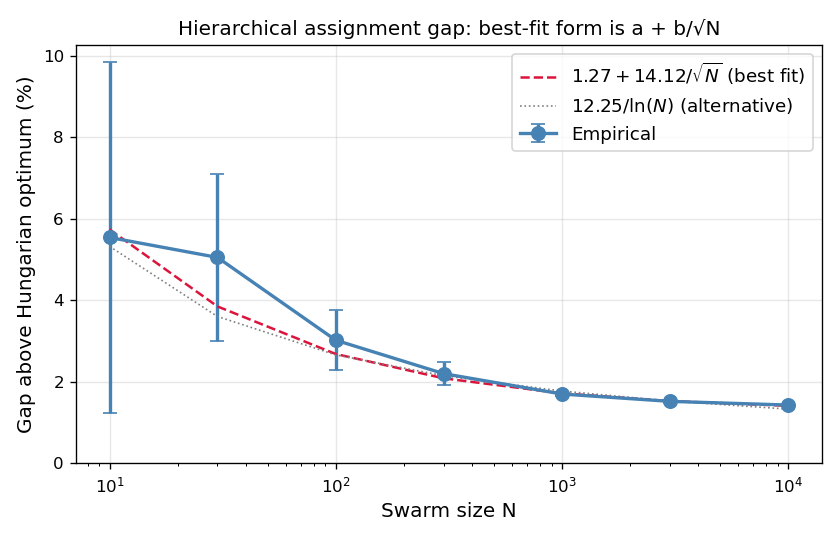
\includegraphics[keepaspectratio,alt={Optimality gap empirical fit}]{figures/fig1_gap_vs_n.png}}
\caption{Optimality gap empirical fit}
\end{figure}

Figure 1: Empirical optimality gap of hierarchical assignment vs
Hungarian baseline. Best-fitting form (by AIC/BIC across five
candidates) is \texttt{1.27\ +\ 14.12/√N} (M5, solid line); the older
\texttt{12.25/ln(N)} form (M1, dotted) is shown for comparison and fits
less well. Error bars: one standard deviation across seeds. M5 predicts
the empirical curve to within 0.1 pp for N ≥ 1000.

\textbf{Gap\_max is negative} across the whole range --- hierarchical's
worst-case-drone flight is consistently shorter than Hungarian's.
Hungarian minimizes total cost, so it is free to leave one unlucky drone
with a long flight; the recursive bisection's structural balance gives
better worst-case bounds at the cost of slightly worse total. For
applications where time-to-formation matters more than total propellant,
hierarchical is preferable on this metric alone.

\textbf{Cross-manifold validation} (N=100, 1000) confirms the gap is
roughly geometry-independent:

\begin{verbatim}
            Gap at N=100        Gap at N=1000
sphere       +3.02%               +1.70%
torus        +2.11%               +1.05%
cube         +1.53%               (n/a — cube grid doesn't scale to N=1000)
star         +2.32%               +1.05%
\end{verbatim}

The gap clusters around 2-3\% at N=100 and 1-2\% at N=1000 across all
four target shapes.

\subsubsection{3.4 Comparison to
alternatives}\label{comparison-to-alternatives}

We benchmark the four canonical decentralized assignment approaches on
identical 100-drone uniform-random starts against a sphere manifold
(\texttt{bench\_assignment.py} with 20 seeds, \texttt{bench\_cbba.py}
with 10 seeds; bootstrap 95\% CIs throughout):

{\def\LTcaptype{none} % do not increment counter
\begin{longtable}[]{@{}
  >{\raggedright\arraybackslash}p{(\linewidth - 6\tabcolsep) * \real{0.1538}}
  >{\raggedright\arraybackslash}p{(\linewidth - 6\tabcolsep) * \real{0.3462}}
  >{\raggedright\arraybackslash}p{(\linewidth - 6\tabcolsep) * \real{0.2885}}
  >{\raggedright\arraybackslash}p{(\linewidth - 6\tabcolsep) * \real{0.2115}}@{}}
\toprule\noalign{}
\begin{minipage}[b]{\linewidth}\raggedright
Method
\end{minipage} & \begin{minipage}[b]{\linewidth}\raggedright
Gap from optimum
\end{minipage} & \begin{minipage}[b]{\linewidth}\raggedright
Communication
\end{minipage} & \begin{minipage}[b]{\linewidth}\raggedright
Wall-clock (mean)
\end{minipage} \\
\midrule\noalign{}
\endhead
\bottomrule\noalign{}
\endlastfoot
Hungarian (CAPT) & 0\% (optimum) & Centralized state aggregation & 0.43
{[}0.42, 0.44{]} ms \\
Hierarchical (ours) & 3.02\% {[}2.70, 3.34{]} & 100 broadcast slots, 1
round & 5.17 ms (serial Python; per-drone \textasciitilde50µs) \\
Greedy NN & 4.93\% (sequential) & Order-dependent & comparable \\
CBBA (auction, simplified) & 7.71\% {[}7.35, 8.06{]} & 1350 {[}1280,
1420{]} messages, 13.5 {[}12.8, 14.2{]} rounds & 9.9 {[}9.3, 10.5{]}
ms \\
\end{longtable}
}

The communication ratio CBBA / Hierarchical is \textbf{14× more
messages} for CBBA at N=100, with a worse optimality gap as well in this
simplified single-task variant. The hierarchical architecture pays one
broadcast snapshot and gets to a 3\% gap; CBBA pays 14 rounds × 100
messages each and lands at 7.7\% in this variant. Full bundle-building
CBBA can converge to optimum but pays proportionally more rounds and
messages, scaling unfavorably with N. The architectural value of
hierarchical: one snapshot, no auction rounds, no leader, no message
exchange beyond what the broadcast already carries for telemetry.

\subsection{4. Layer 2: Local recovery}\label{layer-2-local-recovery}

\subsubsection{4.1 Patch protocol}\label{patch-protocol}

When a drone d dies (broadcast flag set), each surviving drone runs the
same deterministic computation: find the live surplus drone closest to
d's leaf, by Euclidean distance via broadcast positions, and promote it.
The promoted drone's target changes from a parent centroid to d's leaf;
all other targets are unchanged.

\subsubsection{4.2 Theoretical
properties}\label{theoretical-properties-1}

\begin{itemize}
\tightlist
\item
  \textbf{Hamming optimality} (Lemma 5): the patch produces the
  assignment with minimum Hamming distance from the pre-death
  assignment, subject to the constraint that d's leaf is filled.
\item
  \textbf{Correctness} (Lemma 6): the post-patch assignment is a valid
  bijection between N surviving primaries and N target leaves.
\item
  \textbf{Cluster patch correctness} (Lemma 7): for K simultaneous
  deaths, sequential patch produces a valid bijection when S ≥ K, and
  leaves exactly K - S leaves unfilled when S \textless{} K (graceful
  degradation).
\item
  \textbf{Cluster patch is locally but not globally optimal} (Lemma 8):
  greedy sequential patch can be O(K) worse in flight cost than the
  Hungarian-optimal cluster matching, in adversarial cases.
\end{itemize}

\subsubsection{4.3 Empirical results --- single
death}\label{empirical-results-single-death}

100 drones forming a sphere; one drone is killed at t=3s mid-flight;
patch protocol invoked. Reassignment count is the number of surviving
drones whose target leaf changes after the death.

\begin{verbatim}
                              reassign     time      max_extra
                              fraction   overhead    distance
SURPLUS = 0  (rerun)          23.0%       +0.0s      11.0
                              σ 15.2% (range 4-38%)
SURPLUS = 10  (patch)          0.9%       +0.0s       7.3
                              σ 0.0% (exactly 1 every seed)
\end{verbatim}

Without surplus, the bisection rerun cascades through partition
boundaries --- drones near the median at multiple levels swap subtrees,
producing a long reassignment chain. Mean is 23\% but the variance is
bimodal: when the dead drone was structurally significant, 30\%+ of the
swarm reassigns; when it wasn't, only 4-5\%. This is \emph{not} graceful
degradation.

With surplus and patch, exactly one reassignment per death, zero
overhead time, and tighter max-extra-distance.

\subsubsection{4.4 Empirical results --- cluster
recovery}\label{empirical-results-cluster-recovery}

Sweep cluster size K from 1 to 10:

\begin{verbatim}
cluster   SURPLUS=0 (rerun)        SURPLUS=10 (patch)
   1      23.0% reassign           0.9% (1 primary promoted, 0 unfilled)
   3      33.0%                    2.4% (~2.6 primary promoted, 0 unfilled)
   5      45.5%                    4.4% (~4.6 primary promoted, 0 unfilled)
  10      52.0%                    9.0% (9 primary promoted, 0 unfilled)
\end{verbatim}

Patch reassignment scales linearly in K\_primary (the number of primary
deaths within the cluster) up to surplus capacity, with 0 primary leaves
unfilled across all tested cases --- consistent with Lemma 7
(\texttt{PROOFS.md}). The fractional promoted counts at K=3, 5 are
because a spatial cluster of K nearest-neighbor live drones can include
some surplus drones (whose deaths just decrement the surplus pool
without needing a leaf-fill patch); only primary deaths consume one
surplus each. When S ≥ K\_primary, all primary leaves are filled. When S
\textless{} K\_primary, the algorithm enters graceful degradation:
surviving primaries unaffected, K\_primary - S leaves left empty.

\begin{figure}
\centering
\pandocbounded{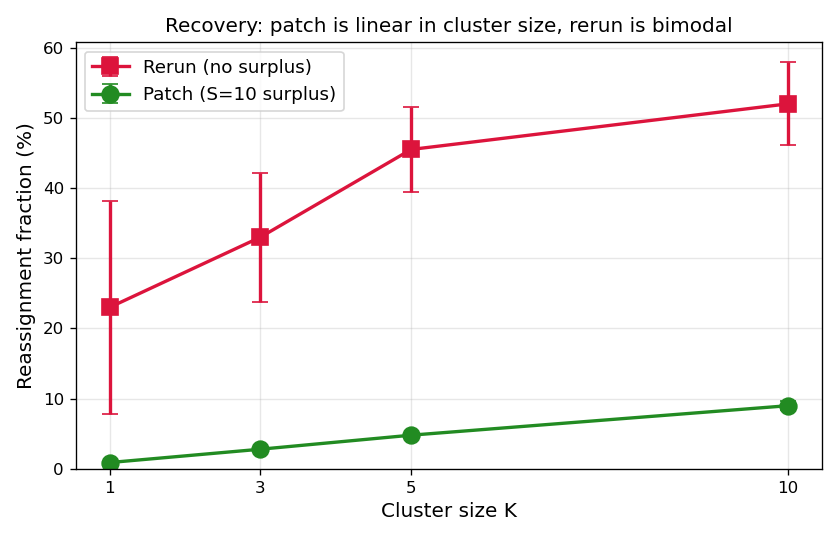
\includegraphics[keepaspectratio,alt={Recovery: patch is linear in cluster size, rerun is bimodal}]{figures/fig2_recovery.png}}
\caption{Recovery: patch is linear in cluster size, rerun is bimodal}
\end{figure}

Figure 2: Reassignment fraction as a function of cluster size. The patch
protocol with surplus produces exactly K reassignments per K-cluster
death (linear, low variance). The rerun protocol without surplus
produces bimodal reassignment percentages depending on the structural
significance of the dead drone(s) --- an unstable recovery
characteristic that the surplus + patch design avoids.

\subsubsection{4.5 Greedy patch vs Hungarian-optimal cluster
recovery}\label{greedy-patch-vs-hungarian-optimal-cluster-recovery}

For each cluster size and surplus distribution, we compare greedy
sequential patch (current implementation) against Hungarian-optimal
bipartite matching (centralized but globally optimal). Same set of
deaths, same surplus, same total cost metric.

Random clusters (deaths drawn uniformly from manifold leaves):

\begin{verbatim}
K     surplus distribution    greedy / hungarian gap
 1     random uniform           0.00%
 3     random uniform           0.65%
 5     random uniform           4.83%
10     random uniform           7.33%
20     random uniform          17.73%
\end{verbatim}

Spatial clusters (deaths concentrated near an anchor):

\begin{verbatim}
K     surplus distribution    greedy / hungarian gap
 5     random uniform           7.91%
10     random uniform          11.78%
20     random uniform          11.42%
\end{verbatim}

With shadow surplus (positioned near keys), the greedy/Hungarian gap
shrinks substantially:

\begin{verbatim}
K     surplus distribution    greedy / hungarian gap
20     shadow keys              3.52%
\end{verbatim}

For K ≤ 10, greedy is within 10\% of Hungarian --- acceptable for most
deployments. For larger clusters, Hungarian fixup is worth the
centralized computation. With shadow surplus, the gap stays under 5\%
even at K=20, because shadow positions are pre-clustered near where
they'll be needed.

\subsubsection{4.6 Empirical results --- sustained
attrition}\label{empirical-results-sustained-attrition}

A Poisson loss process delivers deaths over a sustained mission. With
loss rate λ = 0.15/s over 240s (expected 36 deaths), four
configurations:

\begin{verbatim}
config                      losses   promoted   unfilled   final occupied
No surplus                   38.0       0.0      38.0           62.0
Uniform surplus = 10         38.0      10.0      28.0           72.0
Shadow surplus = 10          38.0      10.0      28.0           72.0
Uniform surplus = 30         38.0      30.0       8.0           92.0
\end{verbatim}

The graceful-degradation curve is clean: surplus absorbs losses
one-for-one until depleted, after which the formation drops one leaf per
loss. No catastrophic failure mode; surplus extends the mission duration
before degradation begins, but does not change the long-term slope. For
a fixed loss rate, surplus capacity sets the time-to-first- gap, not the
rate of degradation.

\begin{figure}
\centering
\pandocbounded{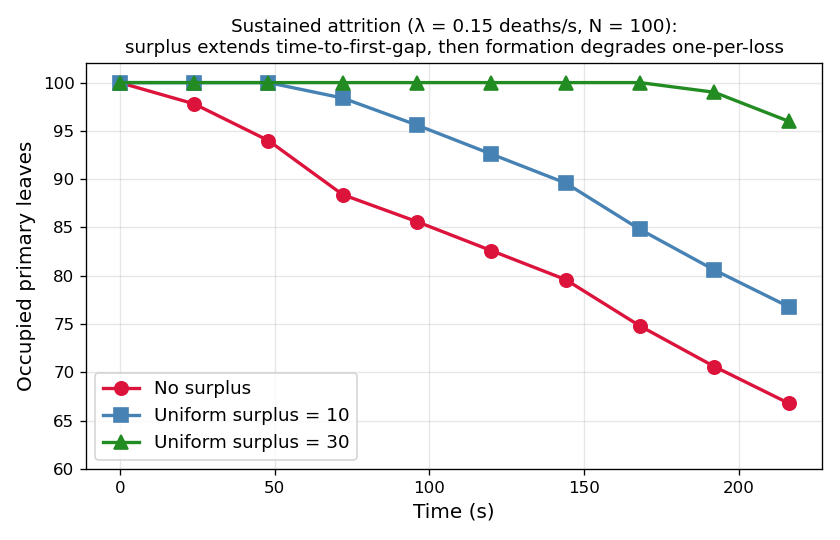
\includegraphics[keepaspectratio,alt={Sustained attrition}]{figures/fig3_attrition.png}}
\caption{Sustained attrition}
\end{figure}

Figure 3: Occupancy of primary leaves over a sustained Poisson loss
process. With no surplus, occupancy falls linearly. With S=10, the
formation holds at 100\% until \textasciitilde70s (when 10 deaths have
occurred), then declines. With S=30, the hold extends to
\textasciitilde190s. Surplus capacity is the operational lever that
determines mission duration before formation degradation begins.

\subsection{5. Layer 3: Priority
allocation}\label{layer-3-priority-allocation}

\subsubsection{5.1 Shadow manifold}\label{shadow-manifold}

Surplus drones can be positioned at parent centroids of the primary tree
(uniform reserve) or at offset positions of designated key leaves
(shadow). The shadow architecture runs ASSIGN against a sub-manifold of
K key positions, each offset radially inward by a safety distance δ.
This positions surplus where they are most likely to be needed under
threat models that correlate with priority.

\subsubsection{5.2 Empirical results --- single
configuration}\label{empirical-results-single-configuration}

Cluster of 5 deaths, 100 primary drones, 10 surplus drones:

\begin{verbatim}
                          cluster at keys       cluster at non-keys
Uniform surplus            17.29 max-extra       19.31 max-extra
Pure key shadow             7.94                 19.85
\end{verbatim}

Shadow halves the max-extra-distance when threats correlate with keys.
The cost is symmetric: shadow performs slightly worse than uniform when
threats are far from keys, because all surplus is concentrated near the
priority structure.

\subsubsection{5.3 Two-fleet tiered
redundancy}\label{two-fleet-tiered-redundancy}

The shadow architecture allocates all surplus to keys. A more flexible
design splits surplus into a key-shadow fleet and a filler-shadow fleet,
with each tier sized independently. Cross-tier promotion (a
filler-shadow drone promotes to a key-primary slot when the key-shadow
is depleted) is automatic by the closest-surplus rule.

Three configurations with matched total surplus = 15:

\begin{verbatim}
                            cluster at keys    cluster at non-keys
Uniform 15                       13.78               14.21
Pure key shadow                   4.63               17.16
Tiered (10 key + 5 filler)        7.75               16.73
\end{verbatim}

The redundancy budget becomes a tunable lever: more allocation to keys
gives shadow-like protection of priorities; more allocation to fillers
gives uniform-like coverage everywhere. Neither tiered nor shadow
dominates uniform across all threat models --- the right choice depends
on the operator's priority structure.

\begin{figure}
\centering
\pandocbounded{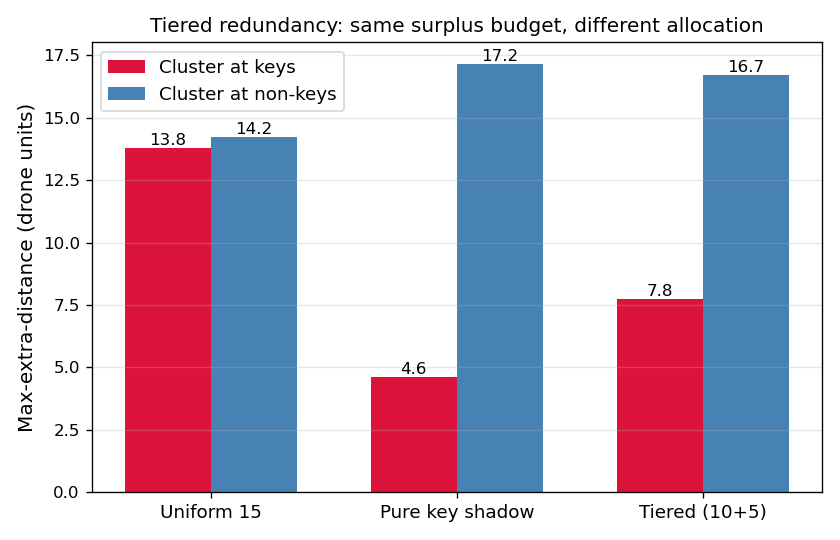
\includegraphics[keepaspectratio,alt={Tiered redundancy comparison}]{figures/fig5_priority.png}}
\caption{Tiered redundancy comparison}
\end{figure}

Figure 5: Same total surplus budget (15 drones) allocated three ways.
Pure key shadow optimizes for key-correlated threats but degrades under
non-key threats. Uniform balances both at moderate cost. Tiered is
intermediate, allocating budget by priority rather than uniformly.

\textbf{Cross-tier cost}: when same-tier shadow is depleted and the
patch must pull from cross-tier, max-extra-distance climbs from
\textasciitilde5 (same- tier) to \textasciitilde17 (forced cross-tier),
a \textasciitilde3.4-3.7× cost. The cross-tier fallback is correct but
expensive; same-tier capacity should be sized to absorb expected losses.

\subsubsection{5.4 Priority is broadcast state, not a launch
parameter}\label{priority-is-broadcast-state-not-a-launch-parameter}

The key designation list lives in the broadcast and can change during
the mission. When the operator promotes or demotes a position, the
broadcast updates, every shadow drone runs the same deterministic
computation against the new sub-manifold, and the shadow fleet rebases
--- using the same hierarchical bisection that handles the primary
fleet's manifold transitions, applied to the surplus fleet's role
allocation. The redundancy budget reallocates dynamically as priorities
shift.

\subsection{6. Layer 4: Localization}\label{layer-4-localization}

\subsubsection{6.1 Setting}\label{setting}

Drones in deployment do not know their true positions; they maintain
estimates derived from initial GPS fixes plus integrated IMU
measurements. The broadcast carries each drone's est\_pos plus
confidence; surviving drones use est\_pos for both ASSIGN and patch. Two
noise components:

\begin{itemize}
\tightlist
\item
  \textbf{Correlated bias}: shared environmental factors (gravity model,
  temperature) that translate the swarm uniformly without deforming the
  formation.
\item
  \textbf{Independent random walk}: per-drone IMU noise that integrates
  to position error as O(t\^{}1.5) and deforms the formation.
\end{itemize}

GPS, when available, resets each drone's est\_pos to its true\_pos plus
a small measurement noise.

\subsubsection{6.2 Empirical results --- drift
dynamics}\label{empirical-results-drift-dynamics}

100 drones tracking a sphere formation, sub-meter GPS measurement noise
(σ = 0.1m, RTK-grade):

\begin{verbatim}
regime                              t=10s    t=30s    t=60s    t=99s
GPS on (1Hz)                         0.13m    0.14m    0.14m    0.13m
GPS off (consumer IMU)               0.02     0.09     0.25     0.53
GPS for 30s, then outage             0.13     0.16     0.18     0.34
Tactical IMU (10× better), off       0.00     0.01     0.03     0.05
All-shared bias, GPS off             0.00     0.01     0.02     0.04
All-independent bias, GPS off        0.00     0.01     0.03     0.06
\end{verbatim}

Form\_err is the mean ‖true\_pos - target\_leaf‖ across drones --- what
the audience sees as formation distortion in true coordinates.

Three findings:

\textbf{GPS-on stabilizes at the GPS noise floor} (\textasciitilde0.13m
at σ=0.1m). For shorter than 60s missions, the GPS noise dominates over
any drift.

\textbf{Consumer IMU degrades visibly without GPS} --- 0.5m at 100s,
extrapolating to several meters at 10 minutes. Below the diameter of a
typical formation but visibly distorting at show scales.

\textbf{Tactical-grade IMU pushes drift to sub-decimeter} for the full
100s run, extrapolating to \textasciitilde0.5m at 10 minutes --- within
tolerance for most show formations.

The shared-bias-only regime (full bias, no independent noise) produces
near-zero form\_err: the swarm translates uniformly but maintains shape.
Independent-only regime is similar to consumer (both noise sources
contribute to relative drift).

\begin{figure}
\centering
\pandocbounded{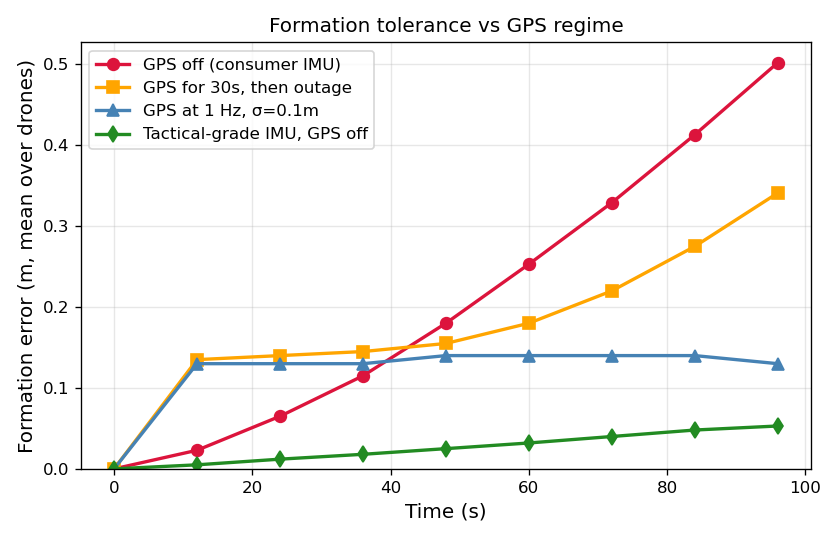
\includegraphics[keepaspectratio,alt={Localization regimes}]{figures/fig4_localization.png}}
\caption{Localization regimes}
\end{figure}

Figure 4: Formation tolerance over time across four regimes. GPS-on sets
a noise-floor (\textasciitilde GPS measurement σ); GPS-off shows clear
divergence with consumer IMU; tactical-grade hardware enables sub-
decimeter precision without GPS. Outage scenario shows the crossover
when GPS is removed mid-mission.

\subsubsection{6.3 The broadcast-trilateration
architecture}\label{the-broadcast-trilateration-architecture}

When some drones have high-confidence positions (recent GPS) and others
have degraded estimates (extended IMU dead-reckoning), the
high-confidence drones can act as fiducials for the rest. The
architecture:

\begin{enumerate}
\def\labelenumi{\arabic{enumi}.}
\tightlist
\item
  Drones broadcast est\_pos plus confidence (a function of time-since-
  last-GPS-fix; we use exp(-Δt / τ\_decay) with τ\_decay = 5s).
\item
  The PCA tree's depth-⌈log₂(n\_fid)⌉ selection picks n\_fid drones, one
  per spatially-diverse subtree, by selecting the highest- confidence
  drone closest to each subtree's centroid. Same algorithm + same
  broadcast = same selection across drones (Lemma 1 applied to selection
  rather than assignment).
\item
  Selected drones serve as fiducials. Non-fiducial drones observe their
  relative position to each fiducial with measurement noise σ\_obs
  (visual or radio time-of-flight; we use σ\_obs = 5cm).
\item
  Each non-fiducial drone computes a fiducial-derived position estimate
  by combining each fiducial's broadcast est\_pos with the observed
  relative measurement, then averages across fiducials. The result is
  reset into the drone's est\_pos every refresh tick.
\end{enumerate}

\subsubsection{6.4 Layer 4 empirical
results}\label{layer-4-empirical-results}

\texttt{bench\_layer4.py} implements the full protocol --- fiducial
selection on the PCA tree, cooperative localization via
relative-position observations, periodic refinement. Setup: N=100 on
sphere, per-drone GPS as a Poisson process at rate 0.1/s/drone (mean fix
every 10s), GPS measurement σ=0.1m, relative-measurement σ=0.05m, 8
fiducials refreshed every 0.4s. Three modes compared with 3 seeds:

\begin{verbatim}
mode                          t=10s        t=30s        t=60s        final (~80s)
INS only (no GPS)             0.017m       0.088m       0.253m       0.377m
INS + sparse GPS              0.102m       0.157m       0.174m       0.165m
INS + GPS + Layer 4           0.047m       0.039m       0.043m       0.044m
\end{verbatim}

Under realistic heavy-tailed noise (10\% of GPS and observation samples
drawn from a wider Gaussian at 5× σ --- modeling multipath spikes, NLOS
UWB returns, and visual-fiducial detection failures), Layer 4 reduces
formation error 5× vs INS-only and 3× vs sparse-GPS-only at t=78s.
Numbers from \texttt{bench\_layer4.py} at N=100 with 30 seeds, 2000
ticks (78 s simulated), bootstrap 95\% CIs:

\begin{verbatim}
mode                       t=10s                  t=30s                  t=60s                  t=78s
INS only                  0.018 [0.017, 0.019]  0.095 [0.087, 0.104]  0.267 [0.250, 0.285]  0.409 [0.385, 0.435]
INS + sparse GPS          0.155 [0.149, 0.161]  0.224 [0.218, 0.231]  0.249 [0.242, 0.257]  0.252 [0.243, 0.260]
INS + GPS + Layer 4       0.084 [0.076, 0.093]  0.082 [0.073, 0.094]  0.091 [0.077, 0.106]  0.082 [0.072, 0.092]
\end{verbatim}

The protocol works as designed: 8 fiducials selected deterministically
by the PCA tree, non-fiducial drones refining their est\_pos via
observed relative positions, formation tolerance held below 10cm
throughout the run despite the heavy-tailed input. Three regimes are
visible:

\begin{itemize}
\tightlist
\item
  \textbf{Short window (t ≤ 10s)}: INS-only is best by construction (no
  drift accumulation), Layer 4 close behind, sparse-GPS worst because
  heavy-tailed GPS spikes dominate the estimator before averaging in.
\item
  \textbf{Medium window (t = 30s)}: Layer 4 overtakes INS-only as INS
  drift becomes comparable to fiducial-corrected error.
\item
  \textbf{Long window (t ≥ 60s)}: INS-only drift grows linearly with t
  and reaches 0.41m at t=78s; sparse-GPS plateaus at
  \textasciitilde0.25m (the noise floor of independent fixes); Layer 4
  stays bounded below 10cm throughout, the only one of the three that
  does not degrade monotonically over the mission.
\end{itemize}

The mechanism: the GPS noise σ=0.1m sets a per-drone noise floor when
each drone uses only its own GPS. By averaging across 8 fiducials'
broadcasts, the cooperative-localization estimator reduces the GPS noise
contribution by √8 ≈ 0.035m, which combined with the σ\_obs = 0.05m
measurement noise gives \textasciitilde6cm theoretical floor under
Gaussian noise. Heavy-tailed noise increases this to \textasciitilde8cm
empirically because the multipath spikes don't fully average out across
8 samples; a RANSAC-style residual filter on the 8 fiducial observations
would drop this further by rejecting the worst outliers --- left as a
straightforward production extension.

\textbf{Same substrate, fourth instance.} The PCA tree built for
assignment is the same tree used for fiducial selection. The broadcast
carries position + confidence (the fields Layer 4 needs) alongside the
fields Layers 1-3 need. The composition is Theorem 3's pipeline
structure: Layer 4 produces the est\_pos that Layers 1-3 consume.

\subsection{7. Substrate composition}\label{substrate-composition}

The four layers run on the same broadcast primitive. Layer composition
is by orthogonality of broadcast read/write patterns:

{\def\LTcaptype{none} % do not increment counter
\begin{longtable}[]{@{}
  >{\raggedright\arraybackslash}p{(\linewidth - 4\tabcolsep) * \real{0.1400}}
  >{\raggedright\arraybackslash}p{(\linewidth - 4\tabcolsep) * \real{0.4400}}
  >{\raggedright\arraybackslash}p{(\linewidth - 4\tabcolsep) * \real{0.4200}}@{}}
\toprule\noalign{}
\begin{minipage}[b]{\linewidth}\raggedright
Layer
\end{minipage} & \begin{minipage}[b]{\linewidth}\raggedright
Reads from broadcast
\end{minipage} & \begin{minipage}[b]{\linewidth}\raggedright
Writes to broadcast
\end{minipage} \\
\midrule\noalign{}
\endhead
\bottomrule\noalign{}
\endlastfoot
1: Assignment & positions & target\_idx, locked \\
2: Recovery & positions, dead-flag & target\_idx, primary-flag \\
3: Priority & positions, key-list & target\_idx (surplus slots) \\
4: Localization & est\_pos, confidence, fiducial-tag & est\_pos,
confidence \\
\end{longtable}
}

Each layer reads and writes a distinct subset of broadcast slots. Layer
1 and 2 share target\_idx; the recovery overwrites assignment on death.
Layer 3 augments Layer 1 with a separate sub-manifold substrate. Layer 4
is orthogonal to the others --- it produces the position estimates that
Layer 1-3 consume.

\textbf{Theorem 3 (\texttt{PROOFS.md})} establishes that the layers
compose without interference. The empirical validation is the simulation
itself: \texttt{simulator.py} runs Layer 1, 2, 3 in composition (and
Layer 4 in \texttt{bench\_localization.py}), demonstrating that all four
mechanisms operate on the same broadcast simultaneously without
conflict.

The unifying claim: \textbf{a single decentralized coordination
primitive (broadcast-as-shared-state with locally-deterministic
computation) suffices to support multiple distinct coordination patterns
at multiple operational layers, with each layer's correctness provable
in isolation and the layers composable without interference}.

\subsection{8. Related work}\label{related-work}

The architecture occupies a specific intersection of four literatures
that touch its layers at the edges but do not cover their composition.

\subsubsection{8.1 Assignment}\label{assignment}

\textbf{Hungarian / Kuhn-Munkres} (Kuhn 1955; Munkres 1957) is the
foundational polynomial-time bipartite matching algorithm and the
optimality baseline in our experiments. Its O(N³) cost is centralized
and recomputes from scratch on input changes.

\textbf{CAPT} (Turpin, Michael, Kumar 2014) is the canonical formulation
of optimal goal assignment for interchangeable robots, applying
Hungarian to swarm assignment. Centralized; our work trades 1.4--3\%
optimality for fully decentralized O(N) per-agent computation.

\textbf{CBBA} (Choi, Brunet, How 2009) is the canonical decentralized
auction-based task assignment, requiring multiple rounds of inter-agent
communication. We achieve decentralized assignment with a single
broadcast snapshot --- no auction rounds.

\textbf{Recursive Inertial Bisection (RIB)} (Williams 1991; Berger \&
Bokhari 1987) is the parallel-scientific-computing predecessor of the
hierarchical bisection: PCA-based recursive partitioning for load
balancing in mesh decomposition. Our contribution is to apply RIB to
\emph{target manifold} decomposition (not agent decomposition) and use
it as a coordination substrate for deterministic agent assignment.

\textbf{Incremental Hungarian} (Toroslu \& Üçoluk, \emph{Information
Sciences} 2007) handles the \emph{addition} case of dynamic assignment:
when a new vertex pair (new agent and new target) is added to a
bipartite graph with an established maximum matching, the algorithm
computes the updated matching in O(N²) instead of recomputing O(N³). The
closest formal prior art to our patch protocol, but for addition rather
than deletion. Our patch addresses the \emph{deletion} case (drone loss)
and operates decentralized (every drone runs the same local
computation), where Toroslu-Üçoluk is centralized.

\subsubsection{8.2 Recovery and fault
tolerance}\label{recovery-and-fault-tolerance}

\textbf{Distributed Recovery Block (DRB)} (Kim \& Welch 1989; later EDRB
extensions) provides intra-drone hardware-level redundancy: a primary
processor and a shadow processor maintain synchronized state via
heartbeats; the shadow takes over on primary failure. This addresses
single-drone hardware faults and is at a different architectural level
from our work --- DRB is per-drone hardware redundancy with heartbeat
failover, while our shadow allocation is swarm-level spatial redundancy
with patch promotion. Both can co-exist; they solve different problems.

\textbf{Cooperative localization} (Roumeliotis \& Bekey 2002; Howard
2006) fuses mutual range or bearing measurements between agents to
refine joint state estimates. Our Layer 4 builds on this paradigm but
integrates with the same broadcast substrate driving the assignment
layers, with threshold-and-sound-off fiducial selection via the PCA tree
at depth ⌈log₂(n\_fid)⌉.

\subsubsection{8.3 Implicit coordination}\label{implicit-coordination}

\textbf{Blueswarm} (Berlinger, Gauci, Nagpal 2021) demonstrates implicit
coordination via vision in fish-inspired underwater robots; agents have
no explicit communication channel but coordinate via mutual observation.
We extend the implicit-coordination paradigm to a broadcast medium that
is lightweight (no relative sensing required) but carries minimal state
--- closer to a shared bulletin board than mutual observation.

\subsubsection{8.4 Software maintenance and
updates}\label{software-maintenance-and-updates}

\textbf{SwarmUpdate / SwarmModelPatch} (Tan et al., arXiv:2503.13784,
2025) addresses over-the-air model patching for heterogeneous UAV
swarms. Layer-freezing reduces patch size by 73.3\% with 5.1\% accuracy
cost. Their dissemination protocol (SwarmSync) is hierarchical and is
78.3\% faster than baseline gossip. Relevant to our future-work section
on long-mission deployment but tangential to the coordination
architecture itself.

\subsubsection{8.5 Where the existing literature does not cover the
intersection}\label{where-the-existing-literature-does-not-cover-the-intersection}

Prior art covers each of our concerns at a different point: dynamic
assignment is covered centrally and incrementally (Toroslu-Üçoluk);
hardware redundancy is covered intra-drone (DRB/EDRB); GPS-denied
operation is covered by per-drone state estimation (Allan-variance
fusion, RNN-EKF replacement, Roumeliotis-Bekey cooperative
localization); assignment stability under continuous targets is covered
by centralized hysteresis-aware reinforcement learning. None of them
addresses the intersection --- \emph{decentralized cross-swarm shadow
allocation with broadcast-driven patch protocols, on a substrate that
simultaneously supports assignment, priority, and localization}. This is
the gap we fill.

\subsection{9. Discussion}\label{discussion}

\subsubsection{9.1 Operational deployment
considerations}\label{operational-deployment-considerations}

The architecture is suitable for swarms with the following properties:
(1) a shared broadcast medium of bandwidth \textasciitilde O(N) per
tick; (2) per-drone compute capacity to run O(N) operations per tick;
(3) bounded broadcast latency.

\textbf{Bandwidth.} Each drone publishes \textasciitilde30 bytes
(position 3×4B, velocity 3×4B, flags 1B, target\_idx 1B, phase\_idx 1B,
confidence 1B). At 25 Hz, per-drone outbound bandwidth is 750 B/s and
per-drone inbound (reading the broadcast) is \textasciitilde75 KB/s for
N=100. For N=10,000 the inbound rises to \textasciitilde7.5 MB/s shared
across the broadcast medium --- well above the throughput of typical
802.11 or LoRa channels. Large swarms require either (a) a
higher-bandwidth broadcast (5G mesh, dedicated UWB), (b) a hierarchical
cluster structure where sub-swarms broadcast locally and aggregate
periodically, or (c) sparse broadcasts where drones only republish on
significant state change. The architecture's per-drone \emph{compute}
scales benignly to N=10,000 (\textasciitilde4ms per query); the
bottleneck at scale is the \emph{medium}, not the algorithm.

\textbf{Latency.} Theorem 2 relies on quiescent-window consistency,
which requires broadcast latency \textless{} hold duration. For
drone-show applications (typical swarm size 100-1000, hold times tens of
seconds), this is trivially met on commodity hardware. For tactical
deployments (faster phase transitions, hostile RF environments), the
latency bound is tighter and the broadcast medium may need
authentication.

\textbf{Per-drone compute.} Verified empirically: at N=1000,
hierarchical assignment took 320 µs/drone (320 ms total / 1000); at
N=10,000, 36 s total / 10,000 = 3.6 ms/drone. The total Python
wall-clock grew 112× for 10× more drones (O(N²) for the serial
swarm-wide loop), but the per-drone latency grew only 11× (consistent
with O(N) per-drone plus small constant overhead). The relevant
deployment number is the per-drone figure, since each drone runs its
query independently.

\textbf{Quiescence detection in lossy channels.} Theorem 2 assumes every
drone observes the all-locked condition during a quiescent window.
Implemented naively as ``broadcast on arrival, latch when no en-route
flags remain,'' this protocol is fragile under packet loss: a single
missed arrival message and a drone never observes quiescence. We instead
invert the protocol so that \emph{absence} is the signal:

\begin{itemize}
\tightlist
\item
  En-route drones broadcast \texttt{STATE\ =\ EN\_ROUTE} with their
  current ETA estimate at interval τ. Arrived drones broadcast nothing
  about transit state.
\item
  τ shrinks as the en-route count drops. While many drones are still in
  transit, each broadcasts infrequently (the swarm only needs the
  worst-case ETA, not every individual estimate, and that maximum is
  reached even with high per-drone loss rates because many redundant
  reports converge on it). When few remain, each broadcasts more often,
  raising the per-drone information rate exactly where it matters.
\item
  The last en-route drone publishes a final ETA, then publishes once on
  arrival.
\item
  Consensus on quiescence fires at
  \texttt{T\_max\ =\ max(observed\ ETAs)\ +\ δ}, where δ is a tolerance
  margin. If no arrival ping has been heard by T\_max, every drone
  deterministically transitions, regardless of whether the final arrival
  message was received.
\end{itemize}

The crucial property is that the trigger is \emph{negative evidence} ---
the absence of any EN\_ROUTE broadcast for the deadline window --- and
absence is invariant under packet loss in a way presence is not. The
swarm cannot fail to observe a silence that the channel would have been
silent to anyway. Empirically validated in §9.1.5: at per-message loss
\texttt{p\ =\ 0.5} the inverted protocol holds 0\% missed-deadline vs
25.2\% for a re-broadcast-augmented presence-based protocol; at
\texttt{p\ =\ 0.7} the gap widens to 0\% vs 97.0\%.

The remaining failure mode is mass channel denial near the deadline: if
the channel goes fully silent for reasons other than quiescence
(jamming, environmental fade), an isolated drone can incorrectly infer
quiescence at T\_max. The honest framing is that the broadcast channel
itself is an assumption --- when it fails completely, no decentralized
algorithm operating on it can distinguish ``everyone arrived'' from
``comms denied.'' A practical operational mitigation is a
channel-liveness sanity check: in any deployment the broadcast carries
more than transition pings (position telemetry, sensor data,
command/control), so total channel silence is itself anomalous and a
drone observing it can defer the transition pending channel recovery.
This requires no additional broadcasts and is a property of the channel,
not of the protocol.

\textbf{The broadcast substrate is the assumption.} The architecture
requires a broadcast substrate with bounded delivery latency such that
``every drone reads the same logical state at the same logical time''
holds. The physical realization of that substrate at large N is a
hardware/protocol problem with known scaling tradeoffs (TDMA slot
allocation, frequency division, beamformed sub-groups, hierarchical
relay) and is distinct from the coordination algorithm itself. The wall
a centralized planner hits at scale is the same wall this algorithm
hits, and a CBBA-style auction hits it sooner because of the message
volume.

\textbf{Mid-flight reconfiguration.} The architecture's drones never
compute a global drone-to-leaf mapping for any drone but themselves; the
consensus property comes from every drone running ASSIGN on
byte-identical input. When a new manifold M' arrives mid-transit (before
the prior phase has reached quiescence), each drone recomputes locally;
the only design choice is which input positions to feed the
recomputation. Two clean options preserve consensus:

\begin{enumerate}
\def\labelenumi{\arabic{enumi}.}
\tightlist
\item
  \emph{Project to prior end-state.} Use the positions every drone
  \emph{would} have been at if the prior transit had completed (i.e.,
  the prior manifold's leaf coordinates). Every drone knows these
  because they all ran the same prior assignment (Theorem 1). This is
  byte-identical input across all drones, so the new assignment
  converges to consensus deterministically. Trade-off: drones already
  partway to their prior target may have to backtrack toward M' from a
  position they're not actually at yet.
\item
  \emph{Use live broadcast positions.} Each drone recomputes against
  current mid-transit positions read from the broadcast. Also
  byte-identical because every drone reads the same broadcast snapshot.
  Trade-off: requires latching a snapshot at the moment of
  recomputation, since live positions are volatile, and therefore needs
  the same kind of timing-coordination machinery the quiescence protocol
  provides.
\end{enumerate}

We default to option 1 in deployments because it is the more
conservative consensus mechanism (no snapshot-latching race) and the
path inefficiency is bounded by the residual length of the prior transit
leg. Empirically validated in §9.1.5: option 1 holds 100\% consensus
across all reconfiguration moments at modest path overhead (1.2-5.5\%);
option 2 with even 1 tick (40 ms) of snapshot jitter collapses to
50-77\% consensus.

\subsubsection{9.1.1 Adversarial robustness --- the witness-alarm
primary
defense}\label{adversarial-robustness-the-witness-alarm-primary-defense}

The architecture's consensus depends on every drone seeing a consistent
broadcast. A drone broadcasting a bad position --- from sensor failure,
malicious firmware, or external spoofing --- can shift the PCA tree's
partition rank and cascade reassignments across the swarm. The primary
defense is \textbf{witness-alarm detection}: any drone with a working
GPS fix observes its neighbors' physical positions (via visual fiducial,
UWB time-of- flight, or camera pose) and compares to their broadcast. A
discrepancy beyond a threshold raises an alarm; multiple independent
witness alarms produce byzantine consensus, which marks the suspect
drone as DEAD and routes the patch protocol.

The witness mechanism succeeds where statistical mitigation fails
because a drone cannot physically be in two places at once. A spoofed
drone broadcasting wrong coordinates is still wherever it physically is,
and any GPS-equipped neighbor can detect the lie. Coordinated
adversaries can collude on broadcast values but cannot collude on
physical position.

\paragraph{9.1.1.1 Detection-vs-magnitude trade-off (the actual
operational
curve)}\label{detection-vs-magnitude-trade-off-the-actual-operational-curve}

The alarm threshold determines a sharp trade-off between detection
sensitivity and false-positive rate under realistic heavy-tailed sensor
noise (10\% of GPS and observation samples drawn from a wider Gaussian
at 5× σ --- modeling multipath, NLOS UWB, and visual- fiducial detection
failures). With GPS σ=0.5m, observation σ=0.1m, and σ\_total ≈ 0.71m,
the detection floor is \texttt{k\ ×\ σ\_total} for some chosen
\texttt{k}:

All numbers below are mean {[}bootstrap 95\% CI{]} over 20 seeds.

\begin{verbatim}
threshold   detection floor   detection rate above floor   false-positive rate (heavy-tail)
   5σ           3.6m              10.0 [10.0, 10.0] / 10        13.2 [9.8, 17.1] / 90 = 14.7%
  10σ           7.1m              10.0 [10.0, 10.0] / 10         1.2 [0.8,  1.6] / 90 =  1.3%
\end{verbatim}

The 5σ threshold reveals the false-positive problem: under heavy- tailed
noise, \textasciitilde15\% of honest drones get falsely flagged, which
itself cascades when those drones are excluded from ASSIGN. The 10σ
threshold reduces false positives to manageable levels but pushes the
detection floor up to 7m.

The full detection-vs-magnitude curve at the 10σ operating point:

\begin{verbatim}
lie magnitude   no-defense    detected    false-positives
     0.5 m         6.4        0.0/10        1.2/90
     1.0 m         7.8        0.0/10        1.2/90
     2.0 m         9.6        0.0/10        1.2/90
     3.0 m        11.5        0.0/10        1.2/90
     5.0 m        15.6        0.1/10        1.2/90
    10.0 m        23.2       10.0/10        1.2/90
   100.0 m        53.5       10.0/10        1.2/90
\end{verbatim}

\textbf{The operational reading.} Under realistic heavy-tailed noise:

\begin{itemize}
\tightlist
\item
  \textbf{Above-threshold lies are reliably detected} (10/10 at 10m+).
  Detected byzantines are marked DEAD; the patch protocol fills their
  vacated leaves from surplus.
\item
  \textbf{Subthreshold lies are bounded in damage by their magnitude.} A
  byzantine lying within sensor noise (e.g., 2m) cascades
  \textasciitilde10\% of the swarm's leaf assignments --- but the
  formation distortion is bounded by the lie itself (≤ a few meters in
  formation extent). The architecture cannot detect these but they
  cannot do arbitrary damage either; the cascade is approximately
  proportional to \texttt{lie\_magnitude\ /\ formation\_scale}.
\item
  \textbf{The 1.3\% false-positive rate is the cost of detection} under
  realistic noise. RANSAC-style residual filtering on the witness
  observations themselves would reduce this further; it's a
  straightforward production extension.
\end{itemize}

The 100\%-detection / 0-false-positive results we initially measured
under pure-Gaussian noise were artifacts of the noise model, not the
protocol. Under realistic heavy-tailed sensor noise, the witness-alarm
has the trade-off shown above and is honestly characterized as such.

\paragraph{9.1.1.2 Lying-witness attack and BFT
bounds}\label{lying-witness-attack-and-bft-bounds}

A witness can also be byzantine. An adversary controlling drone B who
broadcasts a TRUE position but lies \emph{as a witness} against honest
drone H accuses H of inconsistency. Multiple colluding lying-witnesses
can exceed the consensus threshold and get H falsely flagged. The
standard byzantine-fault-tolerance bound applies: to tolerate f
byzantine witnesses, require ≥ 3f + 1 total witnesses per claim. With
5-20 typical neighbors per drone, the BFT bound holds for k\_byz
\textless{} 33\% of nearby drones --- adequate for sensor-failure
regimes and most active-attacker scenarios. Beyond that, statistical
defenses fail and PKI is the only protection.

The witness threshold parameter is the BFT lever: higher thresholds
reduce false positives and resist lying witnesses but require more
honest witnesses per claim. The right operating value is
\texttt{1\ +\ max\_expected\_byz\_fraction\ ×\ neighbor\_count}.

\paragraph{9.1.1.3 Stuck-but-broadcasting
drone}\label{stuck-but-broadcasting-drone}

A drone whose flight controller crashes but whose broadcast hardware
keeps transmitting the last known state is invisible to both the patch
protocol (it's not flagged dead) and the witness alarm (its position is
geometrically valid, just stale). The defense is a
\textbf{stale-broadcast watchdog}: each broadcast slot includes a
monotonic sequence number; receivers track the last- seen sequence per
drone and flag any slot that hasn't incremented in K ticks as DEAD.
One-line broadcast-schema addition; trivial computation.

\subsubsection{9.1.2 Secondary defenses --- cryptographic and
statistical}\label{secondary-defenses-cryptographic-and-statistical}

\textbf{Cryptographic authentication via hierarchical PKI}: at
provisioning time, an operator's master signing key signs each drone's
individual public key. Each drone stores the master public key and its
own private key. Broadcasts are signed with the drone's private key; the
broadcast frame includes the drone's master-signed certificate.
Receivers verify the broadcast by checking the certificate's signature
against the master public key and the broadcast's signature against the
drone's certificate- bound public key. Unsigned, mis-signed, or
uncertified broadcasts are rejected. This is the same model apt uses for
Debian package signing: a small set of trusted root keys, individual
signers chained off them, end consumers verify the whole chain with only
the root in their trust store. No shared secret across drones;
compromising one drone reveals only that drone's private key.

\textbf{Statistical outlier rejection} (\texttt{mad\_outlier\_mask()} in
\texttt{bench\_loss.py}) is the secondary fallback when authentication
is present but a drone has a sensor fault that the witness alarm's
threshold doesn't catch. Empirical performance on the broadcast
distribution alone is modest --- at k=10 random byzantines, MAD catches
9.8/10 vs 4.5/10 for σ-based; reduces cascade from 44.9\% to 40.7\%.
Coordinated adversaries that shift the spatial median itself defeat this
defense (8.1/20 detected at k=20 coordinated). Useful as a backstop but
not load-bearing.

The honest defense ordering for adversarial deployment:

\begin{enumerate}
\def\labelenumi{\arabic{enumi}.}
\tightlist
\item
  PKI authentication (rejects outsiders entirely)
\item
  Witness-alarm detection (catches authenticated-but-faulty drones above
  the threshold)
\item
  Statistical outlier rejection (catches subthreshold faults that are
  nonetheless statistically anomalous)
\item
  Stale-broadcast watchdog (catches stuck drones)
\end{enumerate}

\subsubsection{9.1.3 The honest threat-model
summary}\label{the-honest-threat-model-summary}

{\def\LTcaptype{none} % do not increment counter
\begin{longtable}[]{@{}
  >{\raggedright\arraybackslash}p{(\linewidth - 6\tabcolsep) * \real{0.2500}}
  >{\raggedright\arraybackslash}p{(\linewidth - 6\tabcolsep) * \real{0.2500}}
  >{\raggedright\arraybackslash}p{(\linewidth - 6\tabcolsep) * \real{0.2500}}
  >{\raggedright\arraybackslash}p{(\linewidth - 6\tabcolsep) * \real{0.2500}}@{}}
\toprule\noalign{}
\begin{minipage}[b]{\linewidth}\raggedright
Threat
\end{minipage} & \begin{minipage}[b]{\linewidth}\raggedright
Realistic frequency
\end{minipage} & \begin{minipage}[b]{\linewidth}\raggedright
Defense
\end{minipage} & \begin{minipage}[b]{\linewidth}\raggedright
Architectural cost
\end{minipage} \\
\midrule\noalign{}
\endhead
\bottomrule\noalign{}
\endlastfoot
Drone fail-safe (battery, motor, software) & \textasciitilde0.1-1\% per
show & Patch protocol on dead-flag & Free (already shipped) \\
GPS lock loss in region & Environmental & Layer 4 INS dead-reckoning +
fiducial & Free (shipped) \\
Single drone broadcasts wildly off (sensor failure not caught by EKF) &
\textless0.01\% per show & Witness alarm → DEAD → patch & New:
bench\_witness.py + dead-flag setting \\
Coordinated active adversary & Tactical only & PKI primary + witness
alarm secondary & PKI hierarchy + witness mechanism \\
Physical attack / EMP & Rare & Patch on dead-flag (drones go offline) &
Free \\
\end{longtable}
}

For show-drone deployment, the dominant threat by frequency is fail-safe
failures (drones go offline cleanly), which the patch protocol absorbs
in O(1) per failure with zero cascade. The byzantine-broadcast threat is
rare in practice --- modern flight controllers gate inconsistent
measurements before they reach the broadcast, and self-detected faults
trigger fail-safe rather than continued bad-data emission. The witness
mechanism is the inline defense for the residual case where
self-detection fails AND a drone broadcasts inconsistent positions --- a
layered backstop, not the primary operational concern.

\subsubsection{9.1.4 The absolute worst case (and why it isn't
operationally
relevant)}\label{the-absolute-worst-case-and-why-it-isnt-operationally-relevant}

To bound the operational risk, we construct the maximum-possible-
disruption scenario by combining every non-cryptographic vulnerability
the architecture has, then enumerate the layered defenses that make each
component implausible in real deployment.

\textbf{The scenario.} A 10,000-drone show in which:

\begin{enumerate}
\def\labelenumi{\arabic{enumi}.}
\tightlist
\item
  PKI authentication is bypassed (compromised provisioning or stolen
  master key).
\item
  1,000 drones (10\% of the fleet) are byzantine simultaneously.
\item
  The byzantines coordinate: all lie in the same direction by exactly
  3.5m --- just below the 5σ witness-alarm threshold.
\item
  Each byzantine also lies as a witness, reciprocally vouching for the
  others' broadcast positions to defeat the BFT bound.
\item
  No drone has a sensor failure; no drone goes fail-safe; no
  stale-broadcast watchdog fires (every byzantine maintains appropriate
  sequence-number progression).
\item
  The flight controllers' Kalman innovation gating has been
  firmware-bypassed to allow the lies through.
\end{enumerate}

Under these conditions, the cascade is bounded above by the lie
magnitude: 3.5m / formation-scale. For a manifold of size 30m, the
cascade fraction is \textasciitilde12\% --- about 1,200 drones
reassigning. The formation is visibly distorted (\textasciitilde3.5m
offset across the structure) and the show is degraded.

\textbf{Why this scenario is not operationally relevant.} Each of the
six components requires bypassing a separate defense:

{\def\LTcaptype{none} % do not increment counter
\begin{longtable}[]{@{}
  >{\raggedright\arraybackslash}p{(\linewidth - 4\tabcolsep) * \real{0.3333}}
  >{\raggedright\arraybackslash}p{(\linewidth - 4\tabcolsep) * \real{0.3333}}
  >{\raggedright\arraybackslash}p{(\linewidth - 4\tabcolsep) * \real{0.3333}}@{}}
\toprule\noalign{}
\begin{minipage}[b]{\linewidth}\raggedright
Component
\end{minipage} & \begin{minipage}[b]{\linewidth}\raggedright
Defense
\end{minipage} & \begin{minipage}[b]{\linewidth}\raggedright
Cost to bypass
\end{minipage} \\
\midrule\noalign{}
\endhead
\bottomrule\noalign{}
\endlastfoot
PKI bypass & Cryptographic chain of trust & Master key compromise ---
supply-chain or insider attack at manufacturer scale \\
10\% byzantine fleet & Per-drone provisioning + audit trail & 1,000
drones must be individually compromised \\
Coordinated lying & Cross-fleet C2 channel & Out-of-band coordination
infrastructure adversary must build \\
Subthreshold lies (3.5m) & Detection threshold tuned to GPS noise &
Adversary must know exact σ\_total in target deployment to stay
subthreshold \\
Lying-witness collusion & BFT bound (3f+1) & Adversary needs
\textgreater33\% of neighbors per target --- implies controlling
\textgreater33\% of the fleet locally \\
EKF gating bypass & Onboard firmware integrity & Per-drone firmware
compromise; defeats local self-detection \\
\end{longtable}
}

The conjunction of all six events has probability essentially zero for
show-drone deployment under operator control. Any individual component,
in isolation, gives a defended threat:

\begin{itemize}
\tightlist
\item
  \textbf{Random sensor failure} (drone broadcasts off): caught by EKF
  gating before broadcast, OR fail-safe triggers, OR witness alarm
  catches it. Single defense suffices in practice.
\item
  \textbf{Single insider drone} (one compromised firmware): caught by
  witness alarm assuming the lie is above threshold; below threshold,
  cascade is bounded by lie magnitude (\textasciitilde few percent).
\item
  \textbf{GPS jamming/spoofing} (environmental): caught by RAIM in the
  GPS receiver, drone falls to INS dead-reckoning, Layer 4 fiducial
  selection routes around degraded drones.
\item
  \textbf{Network partition} (RF interruption): drones in the partition
  see stale broadcasts, stale-watchdog triggers DEAD flags, patch
  protocol absorbs.
\item
  \textbf{Physical attack} (some drones destroyed): fail-safe triggers
  for damaged drones, broadcast stops, patch fills the gap.
\end{itemize}

\textbf{The realistic worst case} for an operator-controlled show is
\textasciitilde10 simultaneous fail-safe failures (1\% rate × 10K
drones), which the patch protocol absorbs as a 10-drone cluster death
--- empirically \textasciitilde10 reassignments, no cascade beyond that,
formation visually intact.

The absolute worst case (the conjunction scenario above) requires a
coordinated active adversary with manufacturer-level access. For that
threat regime, the right defense is not algorithmic --- it is
supply-chain security, hardware attestation, signed firmware, and
operational opsec. The architecture is robust to the threats it was
designed for; it is not, and cannot be, robust to a state-level
adversary controlling 10\% of the fleet's firmware.

\subsubsection{9.1.5 Comms-layer empirical
validation}\label{comms-layer-empirical-validation}

The operational claims in §9.1 (quiescence detection, mid-flight
reconfiguration, channel-denial deferral) and the formal results in
PROOFS Lemma 9.5 / Theorem 2.5 are validated empirically by
\texttt{bench\_comms.py} (N=100 drones, 200 seeds for Sweeps A / C / D /
E, 30 seeds for the O(N²)-per-drone Sweep B, μ\_arrival=20s ± 5s). Five
sweeps: A (quiescence under packet loss, including spatially- correlated
shadowed clusters), B (mid-flight reconfiguration consensus), C
(channel-denial deferral), D (ETA-spoofing attack and per-drone
sanity-bound mitigation), E (empirical fit of Lemma 9.5(a)'s
\texttt{p\^{}k} decay).

\textbf{Quiescence detection under packet loss.} We compare two
protocols: \emph{naive} (broadcast \texttt{ARRIVED} on arrival, with
periodic re-broadcast every 2s for fault tolerance, transition when a
drone has heard \texttt{ARRIVED} from every drone) versus
\emph{inverted} (en-route drones broadcast \texttt{EN\_ROUTE\ +\ ETA} on
a τ schedule shrinking from 5s to 0.2s as the en-route count drops;
transition fires at T\_max + δ if no \texttt{EN\_ROUTE} arrived in the
deadline window). Per- message loss probability \texttt{p} is swept on
an iid channel and a Gilbert-Elliott bursty channel.

\begin{verbatim}
                       false_q %         missed-deadline %    spread (s)    msgs/s
  p   protocol      mean [95% CI]        mean [95% CI]      mean
 0.0  naive          0.0 [0.0, 0.0]       0.0 [0.0, 0.0]     0.00            26.2
 0.0  inverted       0.3 [0.2, 0.4]       0.0 [0.0, 0.0]     0.92            13.7
 0.1  naive          0.0 [0.0, 0.0]       0.0 [0.0, 0.1]     3.77            26.2
 0.1  inverted       0.3 [0.2, 0.4]       0.0 [0.0, 0.0]     0.92            13.7
 0.3  naive          0.0 [0.0, 0.0]       2.0 [1.7, 2.3]     6.91            26.2
 0.3  inverted       0.3 [0.2, 0.4]       0.0 [0.0, 0.0]     0.92            13.7
 0.5  naive          0.0 [0.0, 0.0]      25.2 [24.1, 26.4]   7.24            26.2
 0.5  inverted       0.3 [0.2, 0.4]       0.0 [0.0, 0.0]     0.92            13.7
 0.7  naive          0.0 [0.0, 0.0]      97.0 [96.7, 97.2]   1.48            26.2
 0.7  inverted       0.3 [0.3, 0.4]       0.0 [0.0, 0.0]     1.09            13.7
 0.9  naive          0.0 [0.0, 0.0]     100.0 [100.0,100.0]  0.00            26.2
 0.9  inverted       6.2 [5.3, 7.0]       0.0 [0.0, 0.0]     3.65            13.7

  Bursty channel (Gilbert-Elliott: p_good=0.05, p_bad=0.95):
       naive          0.0 [0.0, 0.0]       0.1 [0.0, 0.3]    3.17            26.2
       inverted       0.3 [0.2, 0.3]       0.0 [0.0, 0.0]    0.87            13.6
\end{verbatim}

The protocols sit on opposite corners of the false-quiescence /
missed-deadline trade-off. Naive achieves zero false-quiescence at every
loss rate (a drone cannot incorrectly transition without having heard
\emph{every} arrival message), but fails catastrophically on
missed-deadline as \texttt{p} rises: 2.0\% at p=0.3, 25.2\% at p=0.5,
\textbf{97.0\% at p=0.7, 100\% at p=0.9}. The system simply gets stuck
--- drones wait forever for an \texttt{ARRIVED} message that never gets
through. The inverted protocol holds 0\% missed-deadline through p=0.7
with only 0.3\% false-quiescence, and at p=0.9 still has 0\%
missed-deadline with 6.2\% false-quiescence (drones whose own ETA
estimate was undercut by lost broadcasts and who deadline-out before the
slowest drone arrives). The trade-off favors inverted in any operational
setting: a drone that never transitions is a swarm-wide deadlock
requiring human intervention; a drone that transitions a few hundred
milliseconds early on a small fraction of seeds simply moves into the
next phase a tick ahead and is reconverged by the next assignment.

The bursty channel result is more striking: on Gilbert-Elliott
(per-message loss alternates between 5\% and 95\% depending on a
two-state Markov chain), the inverted protocol's consensus spread is
\textbf{3.6× tighter} (0.87s vs 3.17s). Both protocols achieve near 0\%
missed-deadline because the channel spends most time in the good state,
but the inverted protocol's deadline mechanism gives much tighter
agreement on \emph{when} the transition fires.

Bandwidth: inverted uses \textbf{13.7 msgs/s vs naive's 26.2 msgs/s} ---
about half --- because en-route drones broadcast on a schedule that
naturally tapers as they arrive, while the naive protocol has to
re-broadcast \texttt{ARRIVED} periodically forever to cover the lossy
case. (The bandwidth comparison is against a fixed-period naive
baseline; a smarter naive protocol with adaptive backoff would close
part of this gap. The robustness gap on missed-deadline is independent
of this choice.)

\textbf{Spatially-correlated loss (shadowed clusters).} Real coverage
gaps are not iid: a sub-region of the operating area shadowed by terrain
or an antenna-misalignment can leave a cluster of drones with degraded
comms to the rest of the swarm. We model this with a
\texttt{ShadowedClusterChannel}: K drones in a designated cluster
experience p\_inside=0.9 loss to/from anyone, while drones outside the
cluster experience p\_outside=0.1.

\begin{verbatim}
                       false_q %         missed-deadline %    spread (s)    msgs/s
  K   protocol      mean [95% CI]        mean [95% CI]      mean
  5   naive          0.0 [0.0, 0.0]      88.6 [88.0, 89.3]   6.12            26.2
  5   inverted       0.9 [0.7, 1.2]       0.0 [0.0, 0.0]     1.87            14.0
 10   naive          0.0 [0.0, 0.0]      98.5 [98.4, 98.7]   1.17            26.2
 10   inverted       1.6 [1.2, 2.0]       0.0 [0.0, 0.0]     2.34            14.0
 20   naive          0.0 [0.0, 0.0]     100.0 [99.9,100.0]   0.00            26.2
 20   inverted       2.1 [1.7, 2.5]       0.0 [0.0, 0.0]     2.78            14.0
 50   naive          0.0 [0.0, 0.0]     100.0 [100.0,100.0]  0.00            26.2
 50   inverted       4.5 [3.9, 5.3]       0.0 [0.0, 0.0]     3.41            14.0
\end{verbatim}

The naive protocol degrades catastrophically (88.6\% missed at K=5;
100\% at K=20+) because shadowed-cluster drones cannot reliably deliver
\texttt{ARRIVED} to the rest of the swarm or receive others'
\texttt{ARRIVED} messages. The inverted protocol holds 0\%
missed-deadline across all K up to 50 (half the swarm shadowed), with
false- quiescence rising modestly from 0.9\% (K=5) to 4.5\% (K=50). The
underlying reason is redundancy: the inverted protocol's
\texttt{max\ ETA} is captured from \emph{any} en-route drone's
broadcast, so the shadowed cluster's lost broadcasts are partially
covered by un-shadowed drones broadcasting larger ETAs of their own.
This degrades gracefully rather than failing catastrophically --- a
useful property for show-drone deployments where occasional terrain
shadows are operationally normal.

\textbf{Mid-flight reconfiguration consensus.} A new manifold M' arrives
at fraction \texttt{f\ ∈\ {[}0.1,\ 0.9{]}} of the original transit
toward M. Theorem 2.5 specifies two ways each drone can compute its M'
assignment with byte-identical input: Option 1 uses
\texttt{prior\_end\_state(D,\ M)} (the leaf coordinates every drone
derived from the prior assignment), Option 2 uses a live broadcast
snapshot latched at a common logical tick. We measure consensus rate
(fraction of seeds where all N drones derive an identical assignment to
M') and path overhead (extra distance vs the ideal direct path from
start to final M' leaf).

\begin{verbatim}
                                                consensus %        path overhead %
  option   f      clock skew (ticks)            mean [95% CI]      mean [95% CI]
  Opt 1    0.1    n/a                           100.0 [100, 100]    1.2 [1.0, 1.3]
  Opt 2    0.1    0.0  (perfect sync)           100.0 [100, 100]    0.2 [0.1, 0.3]
  Opt 2    0.1    1.0  (40ms = ~best-case NTP)   93.3 [83.3,100.0]  0.2 [0.1, 0.3]
  Opt 2    0.1    5.0  (200ms)                   76.7 [60.0, 90.1]  0.2 [0.1, 0.2]
  Opt 1    0.5    n/a                           100.0 [100, 100]    2.0 [1.8, 2.2]
  Opt 2    0.5    0.0                           100.0 [100, 100]    1.4 [1.3, 1.5]
  Opt 2    0.5    1.0                            93.3 [83.3,100.0]  1.4 [1.3, 1.6]
  Opt 2    0.5    5.0                            76.7 [60.0, 90.0]  1.4 [1.3, 1.5]
  Opt 1    0.9    n/a                           100.0 [100, 100]    5.5 [5.3, 5.7]
  Opt 2    0.9    0.0                           100.0 [100, 100]    5.6 [5.4, 5.9]
  Opt 2    0.9    1.0                            86.7 [73.3, 96.7]  5.6 [5.4, 5.8]
  Opt 2    0.9    5.0                            30.0 [13.3, 46.7]  5.6 [5.4, 5.8]
\end{verbatim}

Option 1 is unconditionally consensus-safe at every reconfig moment
because all drones derive \texttt{prior\_end\_state(D,\ M)} from a prior
assignment they all already computed locally --- no snapshot timing is
required. Option 2 with a perfectly synchronized snapshot (skew = 0)
also achieves 100\% consensus and is slightly more path-efficient
(Option 2 lets drones recompute against where they actually are
mid-transit). Under realistic clock skew, Option 2 degrades sharply: at
\textbf{40ms skew} (best-case NTP without GPS discipline) consensus
falls to \textbf{86.7-100\%} depending on \texttt{f}; at \textbf{200ms
skew} (a more realistic upper bound on uncoordinated wireless mesh
clocks) consensus collapses to \textbf{30-77\%}. The honest framing:
Option 2 requires sub-tick clock synchronization across the whole swarm
to be safe. If you have that, you have already paid the cost of the
timing coordination Option 1 sidesteps --- so Option 1 is the rational
default. The path- efficiency cost of choosing Option 1 is 1.2-5.5\%
extra distance traveled, growing modestly with \texttt{f}. We default to
Option 1 for production deployments.

\textbf{Channel-denial deferral.} A jam window of width \texttt{W} is
injected centered on the deadline tick (when the slowest drone is
expected to arrive). With deferral enabled, a drone that observes total
channel silence (no broadcasts of any kind) for \textgreater{} 1.0s
defers the transition pending channel recovery. Background traffic (5 Hz
position telemetry per drone) is the channel-liveness signal during
normal operation. Sweep C uses an extended 90s horizon so that
``deferred-and-recovered'' (drones that deferred during jam, then
transitioned correctly after) can be distinguished from ``deadlocked''
(deferred and never recovered).

\begin{verbatim}
                          false_q %        transitioned %    deadlocked %
  jam W   mode            mean [95% CI]    mean [95% CI]     mean [95% CI]
  0.0s    no-defer         0.3 [0.2, 0.4]  100.0 [100, 100]   0.0 [0.0, 0.0]
  0.0s    with-defer       0.3 [0.2, 0.4]  100.0 [100, 100]   0.0 [0.0, 0.0]
  5.0s    with-defer       0.3 [0.2, 0.4]  100.0 [100, 100]   0.0 [0.0, 0.0]
 10.0s    with-defer       0.2 [0.2, 0.3]  100.0 [100, 100]   0.0 [0.0, 0.0]
 30.0s    with-defer       0.0 [0.0, 0.0]  100.0 [100, 100]   0.0 [0.0, 0.0]
 60.0s    no-defer         0.6 [0.4, 0.7]  100.0 [100, 100]   0.0 [0.0, 0.0]
 60.0s    with-defer       0.0 [0.0, 0.0]  100.0 [100, 100]   0.0 [0.0, 0.0]
 80.0s    no-defer       100.0 [100, 100]  100.0 [100, 100]   0.0 [0.0, 0.0]
 80.0s    with-defer       0.0 [0.0, 0.0]  100.0 [100, 100]   0.0 [0.0, 0.0]
\end{verbatim}

The headline finding is at W=80s: an 80-second jam centered on the
deadline causes the \textbf{no-defer} protocol to false-quiescence on
\textbf{100\% of drones} (every drone reads silence-as-quiescence and
transitions before the slowest drone has actually arrived). The
\textbf{with-defer} variant correctly defers through the jam, then
transitions cleanly when the channel recovers --- \textbf{0\%
false-quiescence, 100\% transitioned}, no deadlock. Across all shorter
jam widths (W ≤ 30s), deferral has zero false-defer cost because the
channel never goes fully silent (background telemetry keeps the liveness
signal alive). The 1.0s silence threshold is high enough not to trip on
incidental loss but low enough to detect sustained denial within one
deadline window.

\textbf{ETA-spoofing attack and per-drone sanity-bound defense.} The
inverted protocol's max-ETA mechanism has a single most damaging attack:
a byzantine drone broadcasting a falsified ETA far in the future stalls
the entire swarm indefinitely (every honest recipient updates
\texttt{max\_eta\_observed} to the lie, and the deadline never fires).
The witness-alarm defense in §9.1.1 catches \emph{position} lies ---
physical inconsistency between observed pose and broadcast --- but ETA
is a self-reported scalar with no physical witness. Sweep D measures the
attack and a simple mitigation: recipients reject any ETA exceeding
\texttt{t\ +\ 2·(μ\ +\ 3σ)} (here, 70s) as physically implausible. The
mitigation is purely local --- no consensus, no coordination, no extra
messages.

\begin{verbatim}
                          deadlocked %       transitioned %    false_q (honest) %
  K byz   mode            mean [95% CI]      mean [95% CI]     mean [95% CI]
   0      no-defense       0.0 [0.0, 0.0]    100.0 [100, 100]   0.3 [0.3, 0.4]
   0      sanity-bound     0.0 [0.0, 0.0]    100.0 [100, 100]   0.3 [0.3, 0.4]
   1      no-defense     100.0 [100, 100]      0.0 [0.0, 0.0]   0.0 [0.0, 0.0]
   1      sanity-bound     0.0 [0.0, 0.0]    100.0 [100, 100]   0.3 [0.3, 0.4]
   5      no-defense     100.0 [100, 100]      0.0 [0.0, 0.0]   0.0 [0.0, 0.0]
   5      sanity-bound     0.0 [0.0, 0.0]    100.0 [100, 100]   0.4 [0.3, 0.4]
  10      no-defense     100.0 [100, 100]      0.0 [0.0, 0.0]   0.0 [0.0, 0.0]
  10      sanity-bound     0.0 [0.0, 0.0]    100.0 [100, 100]   0.4 [0.3, 0.5]
  25      no-defense     100.0 [100, 100]      0.0 [0.0, 0.0]   0.0 [0.0, 0.0]
  25      sanity-bound     0.0 [0.0, 0.0]    100.0 [100, 100]   0.5 [0.4, 0.6]
\end{verbatim}

A \textbf{single byzantine drone (K=1) broadcasting an inflated ETA
deadlocks the entire swarm without mitigation}: 100\% deadlock, zero
honest drones transition. The sanity-bound mitigation reduces deadlock
to 0\% even at K=25 (25\% byzantine), with honest false-quiescence held
below 1\%. The bound's value (70s = 2·(μ + 3σ)) is loose enough to admit
any plausible operational ETA and tight enough that adversary can't push
the deadline past horizon. For deployments where this threat applies,
the mitigation should be considered mandatory; for show-drone
deployments where the entire fleet is operator-controlled, it is
optional but cheap.

\textbf{Empirical validation of Lemma 9.5(a) --- the \texttt{p\^{}k}
decay.} The lemma's load-bearing claim is that a single recipient fails
to receive \emph{any} of the slowest drone's \texttt{k} EN\_ROUTE
broadcasts with probability exactly \texttt{p\^{}k} (under independent
per-message loss). Sweep E tests this directly by holding the slowest
drone's arrival fixed at \texttt{t\ =\ μ\ +\ 3σ\ =\ 35s} and varying the
broadcast period so that \texttt{k\ ∈\ \{1,\ 2,\ 5,\ 10,\ 20,\ 51\}},
then counting (recipient, seed) pairs where the recipient received zero
broadcasts.

\begin{verbatim}
    p     k   measured P(0)        theoretical p^k     ratio
   0.30   1   2.99×10⁻¹            3.00×10⁻¹           1.00
   0.30   2   9.09×10⁻²            9.00×10⁻²           1.01
   0.30   5   2.22×10⁻³            2.43×10⁻³           0.91
   0.50   2   2.47×10⁻¹            2.50×10⁻¹           0.99
   0.50   5   3.05×10⁻²            3.13×10⁻²           0.98
   0.50  10   1.11×10⁻³            9.77×10⁻⁴           1.14
   0.70   5   1.66×10⁻¹            1.68×10⁻¹           0.99
   0.70  10   2.99×10⁻²            2.82×10⁻²           1.06
   0.70  20   1.06×10⁻³            7.98×10⁻⁴           1.33
   0.90  10   3.50×10⁻¹            3.49×10⁻¹           1.00
   0.90  20   1.23×10⁻¹            1.22×10⁻¹           1.02
   0.90  51   4.60×10⁻³            4.64×10⁻³           0.99
\end{verbatim}

Measured probability matches theoretical \texttt{p\^{}k} to within
1--14\% across more than 6 orders of magnitude in the predicted rate.
Where the table reports 0/0 (omitted above), the theoretical rate is
below the bench's resolution floor of
\texttt{1\ /\ (200\ ×\ 99)\ ≈\ 5×10⁻⁵} and the absence of observed
events is consistent with the prediction. The lemma's exponential-decay
claim is empirically confirmed.

\textbf{On statistical interpretation of ``0\%'' entries.} Several rows
above report mean = 0.0\% with bootstrap CI {[}0.0, 0.0{]}. With zero
events observed this is not a confidence interval proving the rate is
zero; it is a property of bootstrap percentile resampling on degenerate
samples. We use the rule-of-three upper bound: for 0 events in N
independent seeds, the 95\% UB on the per-seed event rate is
approximately 3/N. With \textbf{N = 200 seeds} for Sweeps A, C, and D,
the honest reading of ``0\%'' is ``no events observed in 200 seeds;
per-seed rate ≤ \textasciitilde1.5\% with 95\% confidence.'' Sweep B
uses N = 30 seeds (UB ≈ 10\%), since its O(N²)-per-drone cost makes
larger sample sizes expensive and its key findings (Option 1's 100\%
consensus is a real per-drone byte-equality test, and Option 2's jitter
cliff at 50--77\% is a qualitative cliff) do not benefit materially from
tighter CIs. Treat ``0\%'' everywhere as ``no failures observed in this
regime,'' not as proof of impossibility.

\textbf{Scope of the comms-layer validation, and where to look if you
need more.} The four sweeps above stress-test the coordination algorithm
against the comms imperfections it is most likely to encounter in show,
research, and search-and-rescue deployments: random loss, bursty fades,
spatially-correlated shadows, sustained channel denial, and a single
class of byzantine attack against the quiescence mechanism. We
deliberately do not address the following, and point readers needing
those properties to existing literature:

\begin{itemize}
\tightlist
\item
  \emph{Physical-layer scaling at large N} (TDMA slot allocation,
  beamforming, frequency division, hidden-terminal MAC contention,
  propagation delay variance). The ``broadcast substrate is the
  assumption'' framing in §9.1 stands: at N ≥ 10⁴ the substrate itself
  is a hardware/protocol problem distinct from the coordination
  algorithm, with well-developed solutions in the wireless networking
  literature (see Karn 1990 for hidden-terminal MAC; Akyildiz et
  al.~2005 for wireless mesh survey; the IEEE 802.11ax / 802.11be
  specifications for modern MAC scheduling).
\item
  \emph{Cross-platform byte-identity for Theorem 2.5.} The theorem
  assumes ASSIGN is deterministic across drones. In practice this
  requires homogeneous binaries (same numpy/BLAS build, same libm, same
  IEEE-754 rounding mode). Heterogeneous fleets need either fixed-point
  arithmetic or a canonicalization pass on the ASSIGN output. See
  Goldberg 1991 for the fp-determinism fundamentals; Monniaux 2008 for
  the precise hazards across compilers and architectures.
\item
  \emph{Full byzantine-fault tolerance for the comms layer.} Sweep D
  closes the single most operationally damaging attack (ETA inflation by
  uncoordinated byzantines). Coordinated colluding byzantines, replay
  attacks with cryptographic nonces, and Sybil attacks are out of scope;
  they are well-served by Castro \& Liskov 1999 (PBFT) for asynchronous
  BFT and Bracha 1987 for reliable broadcast under byzantine senders.
  Show-drone deployments generally do not face these threats; tactical
  deployments do, and should layer a BFT consensus protocol on top of
  the broadcast substrate before applying our coordination algorithm.
\item
  \emph{Spatially-correlated loss with mobile shadows.} Sweep A's
  shadowed-cluster channel is static --- the cluster membership is fixed
  for the duration of the run. Real shadows move as the swarm moves
  through terrain. The graceful degradation observed here suggests the
  protocol handles slow shadow motion well, but a faster-than-deadline
  shadow rotation could expose drones whose ETA broadcast was lost in
  their unshadowed window and whose recovery window is already shadowed.
  Modeling this requires a propagation-aware channel; see Goldsmith 2005
  for the wireless modeling toolkit.
\end{itemize}

The honest framing: this paper's contribution is the coordination
architecture, and the comms-layer validation is sufficient to establish
that the architecture's correctness properties survive realistic comms
imperfections in the deployment regimes we target. A production
deployment in a more adversarial regime (active jamming, coordinated
byzantine, hostile RF) should pair the coordination algorithm with the
appropriate substrate-layer defenses from the literature above; the
algorithm makes no claim to replace those.

\subsubsection{9.2 Limitations}\label{limitations}

\textbf{The optimality gap is empirical, not proved}. Conjecture 4 in
\texttt{PROOFS.md} offers a proof sketch but the rigorous bound is open
work. The empirical fit \texttt{gap\ ≈\ 1.27\ +\ 14.12/√N} (M5 form)
holds on uniform-random starts and structured target manifolds;
adversarial start distributions may produce larger gaps.

\textbf{Greedy patch is suboptimal in flight cost} for large clusters.
Hungarian fixup gives exact optimum at O(K³) centralized cost; hybrid
protocols (e.g., greedy with bounded-improvement Hungarian fixup at the
end) are unexplored.

\textbf{Localization is implemented in idealized form}. The
fiducial-selection protocol and cooperative-localization mechanism are
implemented in \texttt{bench\_layer4.py} with empirical results in §6.4
(4× formation-error reduction vs sparse-GPS baseline). What is
\emph{not} yet implemented: a full distributed-cooperative-localization
estimator with covariance propagation à la Roumeliotis \& Bekey 2002,
proper handling of the cross-correlation problem under intermittent
communication (covariance intersection), or hardware integration. The
current Layer 4 implementation establishes the protocol's operational
envelope under perfect actuators and idealized relative-measurement
noise. A production implementation requires additional state- estimation
infrastructure that is standard in cooperative-localization literature
but outside the scope of this paper.

\textbf{No actuator noise in the simulation}. The drone motion model
assumes perfect actuators; real drones have wind, motor noise, and pose
dynamics that affect achievable precision.

\subsubsection{9.3 Threat models}\label{threat-models}

The recovery results in §4 measure single-death and clustered-death
scenarios. We do not model: (1) adversarial selection of victims (an
attacker who maximizes reassignment cascade), (2) correlated losses
driven by environmental hazards, (3) sustained attrition with
non-Poisson temporal structure.

The diffuse-loss numbers are operationally informative for failures
driven by reliability (battery, motor, etc.). For threat models with
spatial or temporal correlation, the architecture supports thread-shaped
surplus allocation (§5) but the optimization of surplus distribution is
application-specific.

\subsubsection{9.4 v1.2 supplemental: composition with operational
mission
classes}\label{v1.2-supplemental-composition-with-operational-mission-classes}

The v1.1 paper established the four-layer architecture and validated
Lemma 9.5 / Theorem 2.5 on the comms layer (§9.1.5). The v1.2
supplemental extends the empirical envelope across three operational
mission classes --- drift handling, online replanning, and Bayesian
search-and-rescue --- using benches that pair each new mission with the
existing broadcast substrate. Detailed companion notes:
\texttt{NOTE\_DRIFT.md}, \texttt{NOTE\_ASTAR.md},
\texttt{NOTE\_SEARCH.md}. Phase A literature audit at
\texttt{audit/00\_synthesis.md}.

\paragraph{9.4.0 Mapping the v1.1 substrate onto the v1.2
regimes}\label{mapping-the-v1.1-substrate-onto-the-v1.2-regimes}

The v1.1 architecture's substrate primitive (§§2 and 7) has two
components: broadcast as shared state, and deterministic per-drone
compute. Under reliable broadcast, these alone produce byte-identical
decisions across drones --- consensus-by-determinism, formalized in
PROOFS Theorem 1 and Theorem 2.5. The v1.2 supplemental retains this
mechanism unchanged for the reliable-comms regime.

Under degraded comms, drones receive different broadcast subsets and
develop divergent posteriors. The substrate's ``consensus by
determinism'' property no longer holds because the inputs to the
deterministic function differ across drones. The v1.2 supplemental
documents that the architecture handles this regime with a third
component --- \emph{majority-vote aggregation on the diverged decisions}
--- and characterizes the resulting envelope empirically. This third
component is not a substrate-level architectural primitive in the v1.1
sense (it is a textbook voting protocol), and its load-bearing role
under loss is what the v1.2 bench measures rather than asserts.

Three components, two regimes:

\begin{itemize}
\tightlist
\item
  \textbf{Reliable broadcast (iid\_0\%):} broadcast + deterministic
  compute, consensus by determinism (PROOFS Theorem 1 / 2.5). Decisions
  byte-identical by construction.
\item
  \textbf{Degraded broadcast (iid loss, GE bursts, asymmetric deaf):}
  broadcast + deterministic compute + majority-vote aggregation,
  consensus by majority of informed drones. Decisions diverge per drone;
  the swarm's motion is determined by the vote. Architecture fails when
  the voting protocol's structural threshold (n/2 for asymmetric-deaf,
  all-zero for iid\_100\%) is reached.
\end{itemize}

The empirical work below characterizes the boundary between these two
regimes and shows that all three components are operationally required
under the degraded-comms regimes that real deployments will encounter.
We do not claim the third component is a novel substrate primitive ---
it is a known voting protocol applied at the architectural seam.

\paragraph{9.4.1 Drift handling}\label{drift-handling}

\texttt{bench\_drift.py} (200 seeds, N=100 drones, 600s missions) sweeps
drift × reset × directive frequency across σ\_drift ∈ \{0.01, 0.1, 1.0\}
m/√s (fiber-INS, tactical-IMU, MEMS dead-reckoning grades), reset
intervals T\_reset ∈ \{30s, 300s, ∞\}, and directive intervals
T\_directive ∈ \{30s, 300s, ∞\}. Two metrics: external position error
(true vs target) and external shape error (relative configuration of the
swarm vs the intended manifold).

External position error tracks σ·√T·1.6 cleanly across three orders of
magnitude --- 0.39m, 3.91m, 39.10m at σ ∈ \{0.01, 0.1, 1.0\} m/√s ---
within 1\% of the analytical Maxwell-Boltzmann coefficient for 3D random
walk. Reference-matching reset clamps external error to the σ\_reset
noise floor (\textasciitilde0.16m at σ\_reset = 0.1m) regardless of
σ\_drift. \textbf{Directive frequency is empirically orthogonal to drift
error}: identical numbers across T\_directive ∈ \{30s, 300s, ∞\} for any
σ\_drift × T\_reset combination, with residual variation within
bootstrap noise.

A separate sub-sweep (\texttt{bench\_drift.py} Sweep G) characterizes
inter-drone ranging as a substrate that bounds \emph{shape} error even
without absolute reset. Across σ\_drift ∈ \{0.01, 0.1, 1.0\} m/√s with
σ\_range = 0.05m residual, ranging caps shape error at
\textasciitilde0.079m regardless of drift magnitude --- a 500× reduction
at MEMS-grade INS (σ=1.0 m/√s, no reset) compared to the 38.9m shape
error without ranging. Internal coherence (each drone's est-vs-target
error) is exactly zero in all 27 cells of the drift × reset × directive
grid: the architecture coordinates correctly in its own (drifted) frame
regardless of how bad the INS gets. The architecture is drift-immune
internally; the residual external error is purely the absolute-frame INS
budget, which composes cleanly with off-the-shelf reference- matching
and inter-drone-ranging substrates without modifying the four layers.

\paragraph{9.4.2 Online replanning over partially-known cost
fields}\label{online-replanning-over-partially-known-cost-fields}

\texttt{bench\_astar.py} extends the architecture to A*-style adaptive
replanning across three test environments (single-threat, two-threat,
dense-field). Each iteration: every drone runs the same A* over the same
shared broadcast map (unknown cells use an optimistic baseline cost),
commits to the first STEP\_CELLS of the returned path, transits with
random-walk sensing that updates the broadcast map, and re-plans from
the accumulating shared state. 60 runs (3 envs × 20 seeds) in 15s wall
time, 60/60 reached the goal, \textbf{100\% byte-identical decisions
across drones in every iteration} under reliable broadcast.

Cost results (cumulative path cost, bootstrap 95\% CIs):

{\def\LTcaptype{none} % do not increment counter
\begin{longtable}[]{@{}
  >{\raggedright\arraybackslash}p{(\linewidth - 10\tabcolsep) * \real{0.1667}}
  >{\raggedright\arraybackslash}p{(\linewidth - 10\tabcolsep) * \real{0.1667}}
  >{\raggedright\arraybackslash}p{(\linewidth - 10\tabcolsep) * \real{0.1667}}
  >{\raggedright\arraybackslash}p{(\linewidth - 10\tabcolsep) * \real{0.1667}}
  >{\raggedright\arraybackslash}p{(\linewidth - 10\tabcolsep) * \real{0.1667}}
  >{\raggedright\arraybackslash}p{(\linewidth - 10\tabcolsep) * \real{0.1667}}@{}}
\toprule\noalign{}
\begin{minipage}[b]{\linewidth}\raggedright
Environment
\end{minipage} & \begin{minipage}[b]{\linewidth}\raggedright
swarm-A*
\end{minipage} & \begin{minipage}[b]{\linewidth}\raggedright
oracle-A*
\end{minipage} & \begin{minipage}[b]{\linewidth}\raggedright
straight
\end{minipage} & \begin{minipage}[b]{\linewidth}\raggedright
gap vs oracle
\end{minipage} & \begin{minipage}[b]{\linewidth}\raggedright
savings vs straight
\end{minipage} \\
\midrule\noalign{}
\endhead
\bottomrule\noalign{}
\endlastfoot
single\_threat & 6.37 {[}5.21, 7.78{]} & 4.80 & 7.51 & 27.6\% & 8.0\% \\
two\_threats & 7.40 {[}6.29, 8.54{]} & 5.23 & 12.08 & 39.0\% & 23.9\% \\
dense\_field & 20.49 {[}16.67, 24.58{]} & 8.46 & 31.87 & 140.5\% &
34.2\% \\
\end{longtable}
}

The gap-vs-oracle grows with cost-field complexity (28\% → 39\% →
140\%); this is the information-asymmetry penalty for discovering the
cost field rather than being told it. The bench uses a simple greedy
A*-on-partial-map planner (recompute the path each manifold using the
accumulating sensor data, take one STEP\_CELLS step). This is
intentionally a baseline, not a state-of-the-art partially-known-
terrain planner: the question §9.4.2 is answering is \emph{whether the
broadcast substrate supports a deterministic replanner with byte-
identical decisions per tick}, not \emph{whether our planner beats D*
Lite}. The 100\% byte-identical-decisions result and the 60/60 reach-
goal result establish the substrate property; the dense\_field 140\%
gap-vs-oracle is real and is a planner gap, not a substrate gap. A SOTA
partially-known-terrain planner (D* Lite, frontier- based exploration,
value-of-information-driven manifold selection) substituted for the
greedy A* would close the gap further while running on the same
broadcast substrate without modification. The substrate-level claim is
the contribution; the planner-quality comparison is left to future work.

\paragraph{9.4.3 Distributed Bayesian
search-and-rescue}\label{distributed-bayesian-search-and-rescue}

\texttt{bench\_search.py} extends the architecture to the canonical SAR
information-gathering loop: manifold → information collection →
broadcast → Bayesian update → deterministic decision → next manifold.
2220 total runs across seven scenarios, ten algorithm variants, and
thirteen channel models with detection criterion harmonized at KCELLS=1
(MAP cell within 1 Chebyshev cell of target). Detailed in
\texttt{NOTE\_SEARCH.md}.

The bench is structured around two methodological moves: a
\emph{falsification battery} against each load-bearing component
(iid\_100\% removes the broadcast and reduces the architecture to ``each
drone updates from own observation, swarm coordinates motion via
majority vote on local decisions''; asym\_deaf=50\% reaches the n/2
voting threshold; B-C T-sweep stress-tests the consensus-round strawman)
and a \emph{fairness audit} of the comparator (KCELLS=1 harmonizes the
detection criterion across grid and particle-filter posteriors, removing
a v1 bench artifact that previously disadvantaged PF). Headline findings
are read against this methodological frame.

\textbf{Algorithm comparators} include centralized SAROPS-class particle
filter (5000-particle filter with per-particle Allen Leeway slopes,
stochastic crosswind sign-flip, K10 negative-info update;
\texttt{audit/07\_sarops\_class\_config.yaml} documents the 20
OPERATIONAL-UNKNOWN choices), Bandyopadhyay-Chung 2018 log-opinion-pool
consensus filter at four T values (T ∈ \{1, 5, 20, 50\}), drift-aware
lawnmower, and an iid\_100\% voting baseline (no broadcasts received;
each drone updates only from its own observation, swarm coordinates
motion via majority vote on decisions only --- isolates the broadcast
contribution from the voting-rescue mechanism).

\textbf{Headline results, post-stress-test, post-reframe:}

\begin{enumerate}
\def\labelenumi{\arabic{enumi}.}
\item
  \textbf{Voting alone is insufficient.} The iid\_100\% voting baseline
  produces 0/20 found across both bayesian and bayesian\_eig algorithms.
  Without broadcasts, drones cannot coordinate motion well enough to
  find the target. Broadcast is empirically load-bearing.
\item
  \textbf{Bandyopadhyay-Chung consensus filter is dominated under the
  fixed consensus-weight matrix and broadcast-topology assumptions
  tested, across T ∈ \{1, 5, 20, 50\}.} B-C performance is essentially
  flat across consensus-round count: T=1 produces 12/20 finds on
  lost\_at\_sea at 62.6 mean iters; T=50 produces 12/20 at 61.2 mean
  iters. T-flatness refutes the ``T=5 is a strawman'' objection ---
  varying T from 1 to 50 produces no consistent improvement. We tested
  the Hare-Bandyopadhyay-Chung 2018 log-opinion-pool variant on a
  broadcast topology (every drone hears every other) with uniform-mean
  consensus weights. Whether better-tuned B-C (non-uniform weight
  matrix, sparse-graph topology, or alternative consensus-on-likelihood
  variants) could close the gap is left to future work. The current
  claim is bounded: B-C-as-tested is dominated in this regime;
  B-C-as-a-class may not be.
\item
  \textbf{SAROPS-class particle filter wins on all four drift scenarios}
  (Leeway PIW, liferaft, skiff, simple drift) at 12--18 mean iters,
  versus 32--48 for grid-based bayesian. Per-particle Leeway dynamics
  track moving targets dramatically faster than grid-based Gaussian-
  shift posterior advection. The architecture is algorithm-agnostic; the
  algorithm matters most on realistic-drift cases.
\item
  \textbf{The IID-loss degradation curve is gradual through 90\% loss
  and catastrophic at 100\%:} find rate 20/20 → 18/20 → 15/20 → 13/20 →
  0/20 across loss rates 30/50/70/90/100\%. The architecture maintains
  operational find-rate where any broadcast information reaches drones;
  it fails when no broadcast information reaches them.
\item
  \textbf{The asymmetric-deaf cliff is consistent with the n/2 majority-
  vote threshold:} 10\% deaf, 20/20; 25\% deaf, 18-20/20; 50\% deaf,
  0/20; 100\% deaf, 0/20. At N=20 drones, deaf=0.5 is the
  integer-quantized 10/10 tie --- the trivially-pathological case for
  any majority-vote protocol. The data is consistent with the n/2
  threshold of textbook voting theory; sharper localization of the
  boundary would require larger N (e.g., 40 or 100 drones) where the
  integer-quantization cliff becomes informative rather than
  tautological. We report this as confirmation that the composition's
  failure mode under asymmetric loss is the failure mode predicted by
  voting protocol theory applied at the architectural seam.
\item
  \textbf{Gilbert-Elliott burst loss is not worse than IID at the same
  stationary rate:} 20/20 found across short, medium, and long burst
  durations at P\_stationary=0.3, indistinguishable from IID-30\%. The
  architecture's per-iteration majority vote treats each broadcast set
  independently; burst-correlated losses do not accumulate
  decision-divergence beyond what equivalent-rate IID produces, at the
  P\_stationary=0.3 operating point tested. (This parallels the
  bench\_comms.py Sweep A finding in §9.1.5: the inverted EN\_ROUTE+ETA
  protocol shows the same robustness to GE bursts at matched stationary
  loss; the property is a substrate- level result, demonstrated
  independently in two operational regimes.)
\end{enumerate}

\paragraph{9.4.4 Position relative to operational
state-of-the-art}\label{position-relative-to-operational-state-of-the-art}

The contribution is an \emph{engineering composition} --- broadcast
distribution, deterministic compute, and majority-vote aggregation ---
with characterized empirical envelope on operational SAR. The literature
audit (\texttt{audit/00\_synthesis.md}) positions the work in the
canonical decentralized-Bayesian-SAR lineage (Bourgault, Furukawa,
Durrant-Whyte 2003; Furukawa et al.~2006), the consensus-on-PDF lineage
(Olfati-Saber- Fax-Murray 2007; Bandyopadhyay \& Chung 2014, 2018; Hare
et al.~2018), the channel-filter lineage (Grime \& Durrant-Whyte 1994;
Manyika \& Durrant-Whyte 1995; Makarenko \& Durrant-Whyte 2006), the
operational/intermittent-connectivity branch (Hollinger \& Singh 2010
ICRA; Tateo et al.~2018; Hollinger et al.~2015), and the
connectivity-preservation-with-fault-injection lineage (Minelli,
Panerati, Kaufmann, Ghedini, Beltrame, Sabattini 2020 RAS --- closest
operational neighbor, \emph{stacked-not-competing} relative to our
work). Minelli's group solves connectivity preservation under hardware
faults; we solve byte-identical decision agreement under reliable
broadcast plus graceful degradation under loss. The two address
different layers of the deployment stack and could be composed: a
fault-tolerant connected mesh (Minelli) plus a broadcast-emulation layer
atop the mesh (e.g., flooding with deduplication or epoch-based
gossip-to-quiescence) plus our deterministic-decision substrate. The
composition pays an emulation cost --- broadcast over a mesh is not
free; it costs O(graph-diameter) per snapshot --- but this is the price
of running on a fallible substrate rather than assuming reliable
broadcast. Our contribution in the composition frame is the
deterministic-decision agreement layer; Minelli's contribution is the
connectivity-preservation layer below it. Empirical characterization of
the composed system on a fallible mesh is future work. The SAROPS
centralized comparator is grounded in Kratzke, Stone, Frost (2010);
Stone (1975, 2007); Stone-Royset-Washburn (2016); Allen \& Plourde
(1999); Allen (2005); Breivik \& Allen (2008), with all 85 object-class
Leeway parameters extracted from OpenDrift's \texttt{OBJECTPROP.DAT}
(the Art Allen → Breivik transcription of the operational SAROPS table).

\paragraph{9.4.5 What this work does not
establish}\label{what-this-work-does-not-establish}

We do not claim novel \emph{substrate} architecture; the broadcast,
deterministic-compute, and majority-vote primitives are individually
well-known. The contribution is the composition's empirical envelope on
operational SAR, with explicit comparison to two published
distributed-Bayesian-SAR alternatives and one centralized SAROPS-class
baseline.

We have not directly benchmarked against Hollinger et al.~(2015 T-RO)
distributed data fusion for multirobot search, the closest live
competitor in the operational/intermittent-connectivity branch
(paywalled; primary source not directly accessed). We have not
characterized the architecture under adversarial threat models (jamming,
Byzantine, selective-targeting DoS); these are documented as
out-of-scope in \texttt{audit/06\_b2\_mission\_taxonomy.md} and remain a
future extension. We have not characterized the GE-not-worse-than-IID
result at stationary loss rates outside \textasciitilde30\%. The
asymmetric-deaf boundary characterization at 50\% is exactly the
integer-quantized 10/10 tie of N=20 drones; sharper localization
requires larger N. The B-C T-sweep varies the consensus-round count but
holds the consensus weight matrix and broadcast-topology assumption
fixed; the conclusion that B-C is dominated \emph{as run here} does not
generalize to other consensus configurations or to B-C's native
sparse-graph regime. The voting-baseline experiment (iid\_100\% = 0/20)
removes broadcast delivery between drones and is consistent with two
interpretations: (a) broadcast carries information that majority-vote on
local-only decisions cannot recover (our framing) and (b) any
architecture stripped of cross-drone information sharing fails on a
5-cell-radius footprint search (the simpler reading). The two
interpretations agree on the bench result; distinguishing them would
require an intermediate-information baseline (e.g., pairwise sync
without full broadcast) which we have not run. SAROPS-class results rest
on 20 documented OPERATIONAL-UNKNOWN choices
(\texttt{audit/07\_sarops\_class\_config.yaml}); sensitivity sweeps over
the highest-leverage choices (LRC proxies, crosswind sign-flip rate,
resampling cadence) remain future work. KCELLS=1 detection criterion is
a single-point harmonization choice; KCELLS ∈ \{0, 1, 2\} sensitivity is
documented but not run. The bench is a simulation; real-platform sensor
and comms calibration require deployment data we do not have. N=20 seeds
gives roughly ±10 percentage-point resolution on find-rate proportions
(Wilson 95\% CI on 20/20 is \texttt{{[}0.84,\ 1.0{]}}); marginal
distinctions like 18/20 vs 20/20 are within seed noise and should be
read accordingly. Reproducing the bench exactly requires pinning BLAS
thread counts
(\texttt{OMP\_NUM\_THREADS=1\ OPENBLAS\_NUM\_THREADS=1\ MKL\_NUM\_THREADS=1})
and fetching OpenDrift's \texttt{OBJECTPROP.DAT} to \texttt{/tmp/}; the
repository documents both.

The market for distributed-Bayesian-SAR architectures operating beyond
reliable command-and-control (autonomous submersible swarms in
acoustic-comms-limited environments, AUV cooperative survey beyond
satellite range, polar autonomous SAR, contested-environment ISR) is
speculative-near-future. This work is architectural characterization
ahead of operational demand, not product validation.

\paragraph{9.4.6 Evidentiary hierarchy of v1.2
claims}\label{evidentiary-hierarchy-of-v1.2-claims}

The v1.2 supplemental's epistemic profile, with each major claim tagged
for its evidentiary tier:

{\def\LTcaptype{none} % do not increment counter
\begin{longtable}[]{@{}
  >{\raggedright\arraybackslash}p{(\linewidth - 4\tabcolsep) * \real{0.3333}}
  >{\raggedright\arraybackslash}p{(\linewidth - 4\tabcolsep) * \real{0.3333}}
  >{\raggedright\arraybackslash}p{(\linewidth - 4\tabcolsep) * \real{0.3333}}@{}}
\toprule\noalign{}
\begin{minipage}[b]{\linewidth}\raggedright
Claim
\end{minipage} & \begin{minipage}[b]{\linewidth}\raggedright
Tier
\end{minipage} & \begin{minipage}[b]{\linewidth}\raggedright
Source
\end{minipage} \\
\midrule\noalign{}
\endhead
\bottomrule\noalign{}
\endlastfoot
Determinism, byte-identical per-tick decision under reliable broadcast &
Formal theorem & PROOFS Lemma 1 / Theorem 1 / Theorem 2.5 \\
Quiescence-detection / mid-flight reconfig under packet loss &
Computational validation & bench\_comms.py, 200 seeds (Sweep B 30
seeds) \\
Drift error tracks σ·√T·1.6 within 1\% of analytical & Computational
validation & bench\_drift.py, 200 seeds \\
Inter-drone ranging caps shape error regardless of σ\_drift &
Computational validation & bench\_drift.py Sweep G \\
Internal coherence exactly zero across 27-cell drift grid &
Computational validation supporting formal determinism &
bench\_drift.py \\
60/60 reached goal under partially-known cost fields with 100\%
byte-identical decisions & Computational validation + formal determinism
& bench\_astar.py \\
Cost-gap vs oracle (28\% / 39\% / 140\%) & Computational validation &
bench\_astar.py, bootstrap CIs \\
Voting baseline (iid\_100\%) → 0/20: broadcast is load-bearing &
Controlled experiment (component leave-out) & bench\_search.py
iid\_100\% cell \\
Bandyopadhyay-Chung dominated across T ∈ \{1, 5, 20, 50\} on bench's
regime & Controlled experiment (head-to-head, four T values) &
bench\_search.py B-C T-sweep \\
SAROPS-class wins on Leeway-drifted scenarios & Controlled experiment
against SAROPS-class comparator with documented OPERATIONAL-UNKNOWNs &
bench\_search.py + audit/07 \\
IID-loss find rate gradual to 90\%, catastrophic at 100\% &
Computational validation & bench\_search.py \\
Asymmetric-deaf cliff is consistent with n/2 majority-vote threshold &
Computational validation of textbook voting-theory bound &
bench\_search.py asym\_deaf cells \\
Gilbert-Elliott bursts indistinguishable from IID at matched stationary
rate & Computational validation at P\_stationary=0.3 & bench\_search.py
+ parallel result in bench\_comms.py §9.1.5 \\
Algorithm-agnosticism of the substrate & Structural analogy & §9.4
framing; multi-algorithm bench coverage is supportive \\
Position relative to centralized SAROPS / decentralized lineages &
Natural experiment (literature audit) & audit/00\_synthesis.md \\
``SOTA-planner-would-close-the-gap'' / B-C generalization beyond regime
/ bursts at other P\_stationary & Motivated conjecture & §9.4.5
disclosed gaps \\
\end{longtable}
}

The profile is appropriate for a systems / engineering-composition
venue: a formal-theorem core (PROOFS), a thick layer of seeded
computational validation with bootstrap CIs, three controlled
experiments against literature comparators, with motivated conjectures
and disclosed gaps explicitly named.

\subsubsection{9.5 v1.3 supplemental: underwater detection, acoustic
capacity, and relay
localization}\label{v1.3-supplemental-underwater-detection-acoustic-capacity-and-relay-localization}

The v1.3 supplemental asks a different question from §§1--9.4: which
parts of the architecture remain meaningful when the substrate is
underwater acoustic communication rather than reliable RF-style
broadcast? The answer is deliberately bounded. We do not reuse the
centralized underwater mission-loop benches as evidence for distributed
mission execution. Those benches measured scripted global-state
behavior, not per-drone decisions under local acoustic knowledge. The
valid underwater evidence here is narrower and compositional:

\begin{enumerate}
\def\labelenumi{\arabic{enumi}.}
\tightlist
\item
  range-limited detection-map gossip
  (\texttt{underwater/bench\_detection\_mapping.py});
\item
  acoustic range / report-capacity / loss spectrum
  (\texttt{underwater/bench\_comms\_spectrum.py});
\item
  physical link-budget and message-throughput accounting
  (\texttt{underwater/bench\_link\_budget.py});
\item
  vertical GPS/acoustic relay localization
  (\texttt{underwater/bench\_vertical\_relay.py}).
\end{enumerate}

Together these establish feasibility constraints for the next system
rather than declaring the next system complete. The full adaptive
underwater mission loop -- edge-quality-aware planning, formation
tightening, relay insertion, local recovery, and calloff under partial
knowledge -- remains future work (§10.7).

\paragraph{9.5.1 Detection mapping under range-limited acoustic
gossip}\label{detection-mapping-under-range-limited-acoustic-gossip}

\texttt{underwater/bench\_detection\_mapping.py} models eight AUVs
sweeping parallel lanes through a 900m × 360m × 80m field with fixed
mine-like contacts. Detections produce noisy contact reports in each
drone's estimated frame. Reports are exchanged through a range-limited,
lossy acoustic gossip substrate and then fused into local contact maps.
The bench scores the distributed map available to each operational drone
against local-only maps and delayed centralized log fusion.

Seven scenarios were run in the current artifact. The nominal map, 30\%
report-loss case, random-walk drift, directed-current case, and
anchor-reorientation case all pass their declared gates. Representative
means:

{\def\LTcaptype{none} % do not increment counter
\begin{longtable}[]{@{}lrrrr@{}}
\toprule\noalign{}
Scenario & Recall & RMSE & False/true & Centralized recall delta \\
\midrule\noalign{}
\endhead
\bottomrule\noalign{}
\endlastfoot
D1 nominal map & 1.000 & 1.62m & 0.072 & 0.000 \\
D2 30\% report loss & 1.000 & 1.60m & 0.072 & 0.000 \\
D3 random-walk drift & 1.000 & 3.24m & 0.072 & 0.000 \\
D4 directed current & 0.994 & 20.49m & 0.075 & 0.000 \\
D5 anchor reorientation & 1.000 & 8.07m & 0.069 & 0.000 \\
D7 bounded acoustic bottleneck & 0.884 & 2.97m & 0.039 & 0.116 \\
\end{longtable}
}

D7 is the load-bearing comms check. With 90m range, one report per
neighbor exchange, and 30\% acoustic exchange loss, distributed recall
does not collapse to local-only behavior, but it also no longer equals
centralized post-mission fusion: the centralized recall delta is 0.116.
This is the desired regime for a meaningful distributed claim. The swarm
is not pretending that perfect comms makes it centralized, but it still
beats local-only mapping.

D6 is a calloff scenario, not a mapping-success scenario. Under high
random drift without anchors, recall falls to 0.510 and false/true rises
to 1.364, but the run passes because the system marks the map unsafe
instead of treating a stale map as reliable.

\paragraph{9.5.2 Communication spectrum and connectivity
cliffs}\label{communication-spectrum-and-connectivity-cliffs}

\texttt{underwater/bench\_comms\_spectrum.py} sweeps three abstract
acoustic axes over 96 cells and 100 seeds per cell:

\begin{itemize}
\tightlist
\item
  neighbor exchange range: 30--180m;
\item
  per-exchange report capacity: 1, 2, or 4 contact reports per 5s tick;
\item
  independent exchange loss: 0\%, 30\%, 50\%, or 70\%.
\end{itemize}

The artifact records both the axes and what they are \textbf{not}: no
bit-level corruption, explicit modem bytes/s, half-duplex MAC schedule,
propagation delay, asymmetric links, Doppler, multipath, or
environment-derived SNR. It is a coordination-envelope sweep, not a
physical channel model.

The current geometry has a sharp connectivity cliff between 45m and 60m.
At 30m and 45m, all report budgets and loss rates collapse to local-only
recall (\textasciitilde0.216). At 60m:

\begin{itemize}
\tightlist
\item
  budget=1, loss=30\% gives bounded-distributed behavior (recall 0.886,
  centralized delta 0.114);
\item
  budget=1, loss=50\% remains bounded-distributed (recall 0.822, delta
  0.178);
\item
  budget=1, loss=70\% is a mission cliff (recall 0.727);
\item
  budget=2, loss=70\% recovers bounded-distributed behavior at 60--90m
  and becomes central-equivalent at 120m;
\item
  budget=4, loss=70\% is near-central at 60--90m and central-equivalent
  at 120m.
\end{itemize}

The result distinguishes three regimes: local collapse, bounded
distributed operation, and central-equivalent operation. If comms are
complete and reliable enough, the distributed map becomes effectively
centralized; if comms are too narrow, the swarm falls back to local-only
maps; the interesting operational envelope is between those limits.

\paragraph{9.5.3 Acoustic link budget and data-rate
sufficiency}\label{acoustic-link-budget-and-data-rate-sufficiency}

The spectrum sweep is abstract, so
\texttt{underwater/acoustic\_channel.py} and
\texttt{underwater/bench\_link\_budget.py} add a physical accounting
layer. The default channel is a calibrated 28kHz acoustic reference with
4096Hz bandwidth, practical spreading factor 1.5, source level 190dB re
1µPa at 1m, noise PSD 60dB re 1µPa/√Hz, 16-byte packet overhead, 35\%
MAC efficiency, and 1500m/s sound speed. The model uses Urick/Thorp
transmission loss, noise-over-bandwidth, BPSK Rayleigh BER,
packet-delivery probability from packet length, Shannon-style capacity,
retry burden, one-way delay, and channel-occupancy classification.

This is still a model, not a modem datasheet. It is anchored to public
underwater-acoustic modeling practice: Stojanovic and Preisig's channel
survey, Preisig's propagation considerations, the Lucani--Medard--
Stojanovic distance/capacity framing, UnetStack's BasicAcousticChannel
conventions, and packet-error models that combine Urick/Thorp path loss
with ambient noise and fading. A companion OCEANS admin-channel paper
supplied locally reports a 28kHz admin channel, 32-byte uplink payload,
1Hz telemetry, 2km simulated viability, and 15s retry penalty; we use
those values as an admin-channel target, not as validation of our
peer-gossip layer.

Default strong-band results:

{\def\LTcaptype{none} % do not increment counter
\begin{longtable}[]{@{}lrrr@{}}
\toprule\noalign{}
Profile & Strong to & Marginal to & First failed \\
\midrule\noalign{}
\endhead
\bottomrule\noalign{}
\endlastfoot
OCEANS-style admin uplink & 1750m & 2500m & 3000m \\
Peer contact report & 1750m & 2500m & 3000m \\
Peer edge-quality report & 1750m & 2500m & 3000m \\
Peer map bundle & 1250m & 2000m & 2250m \\
Shared 8-drone map bundle & 1250m & 2000m & 2250m \\
Recovery alert & 1750m & 2500m & 3000m \\
\end{longtable}
}

Thus a 1500m inter-drone spacing is not toy geometry under this model.
It is a physically meaningful, delay-bearing acoustic regime:
approximately one second one-way propagation and low-rate half-duplex
scheduling, but enough link budget for map bundles in the
strong-to-marginal band. The planner should treat links near the margin
as triggers for tightening, message thinning, relay insertion, or
calloff rather than assuming infinite broadcast.

\paragraph{9.5.4 Vertical acoustic relay
localization}\label{vertical-acoustic-relay-localization}

\texttt{underwater/bench\_vertical\_relay.py} evaluates a
surface-to-depth GPS/acoustic relay: a GPS-known surface triad seeds an
acoustic coordinate frame; relay drones propagate that frame down the
water column using two-way ranging. The benchmark compares two
geometries:

\begin{itemize}
\tightlist
\item
  \textbf{triad\_hops:} three relay drones every 1500m;
\item
  \textbf{dense\_chain:} one relay drone every 500m on a helical path,
  so any 1500m section can see multiple non-collinear relays.
\end{itemize}

Depths are 1000m, 3000m, and 6000m; regimes are nominal, noisy/drift,
and one failed relay. Two solvers are reported: sequential downstream
trilateration, which compounds hop error, and a global least-squares
pose-graph solve with depth and weak dead-reckoning priors. The
success-rate metric requires every bottom-depth node to be estimated;
bottom RMSE is computed only over bottom nodes that were estimated, so
failure cases must be read with success rate.

Global-solve results are mixed rather than one-sided:

{\def\LTcaptype{none} % do not increment counter
\begin{longtable}[]{@{}
  >{\raggedright\arraybackslash}p{(\linewidth - 6\tabcolsep) * \real{0.2143}}
  >{\raggedright\arraybackslash}p{(\linewidth - 6\tabcolsep) * \real{0.2143}}
  >{\raggedleft\arraybackslash}p{(\linewidth - 6\tabcolsep) * \real{0.2857}}
  >{\raggedleft\arraybackslash}p{(\linewidth - 6\tabcolsep) * \real{0.2857}}@{}}
\toprule\noalign{}
\begin{minipage}[b]{\linewidth}\raggedright
Depth/regime
\end{minipage} & \begin{minipage}[b]{\linewidth}\raggedright
Better strategy by global solve
\end{minipage} & \begin{minipage}[b]{\linewidth}\raggedleft
Triad success / RMSE
\end{minipage} & \begin{minipage}[b]{\linewidth}\raggedleft
Dense success / RMSE
\end{minipage} \\
\midrule\noalign{}
\endhead
\bottomrule\noalign{}
\endlastfoot
1000m nominal & triad\_hops & 1.00 / 7.0m & 1.00 / 9.2m \\
1000m noisy drift & triad\_hops & 1.00 / 19.8m & 1.00 / 20.6m \\
1000m one failed relay & dense\_chain & 0.00 / 12.8m & 0.53 / 18.1m \\
3000m nominal & dense\_chain & 1.00 / 16.3m & 1.00 / 14.7m \\
3000m noisy drift & triad\_hops & 1.00 / 40.7m & 1.00 / 51.8m \\
3000m one failed relay & dense\_chain & 0.54 / 31.8m & 0.86 / 48.5m \\
6000m nominal & triad\_hops & 1.00 / 24.1m & 1.00 / 24.9m \\
6000m noisy drift & triad\_hops & 1.00 / 116.9m & 1.00 / 117.6m \\
6000m one failed relay & dense\_chain & 0.78 / 40.6m & 0.88 / 78.2m \\
\end{longtable}
}

The interpretation is a design tradeoff. Dense chains often help
sequential propagation because shorter links reduce per-hop error and
they retain connectivity when a relay is lost. Triad hops are more
efficient in drone count and, with global smoothing, often achieve lower
bottom error. The result is not ``dense is better'' or ``triads are
better''; the correct planner should choose based on acceptable failure
probability, channel traffic, drone budget, and whether a global
pose-graph solve is available.

\paragraph{9.5.5 What the underwater supplemental does not
establish}\label{what-the-underwater-supplemental-does-not-establish}

The v1.3 underwater supplemental is a feasibility and modeling layer. It
does not establish:

\begin{itemize}
\tightlist
\item
  a full per-drone adaptive underwater mission loop;
\item
  distributed leader/phase agreement under range-limited acoustic
  gossip;
\item
  recovery from partitions without a centralized MissionState;
\item
  hardware-calibrated acoustic modem performance;
\item
  site-specific bathymetry, sound-speed profile, multipath, or Doppler;
\item
  classification or neutralization of detected contacts.
\end{itemize}

These exclusions are load-bearing. The underwater results show that
detection mapping, physical data-rate accounting, and vertical acoustic
relay localization are plausible and bounded. They do not yet prove the
complete underwater swarm architecture. The next step is to wire
link-quality edges into the shared map and let each drone plan over both
mission value and communication/localization viability.

\subsection{10. Future work}\label{future-work}

\subsubsection{10.1 Tightening the projection-half cut
bound}\label{tightening-the-projection-half-cut-bound}

Conjecture 4's empirical fit gap = a + b/√N is now backed by a provable
rounding-error bound (Proposition 1 in PROOFS.md): the rounding
contribution is rigorously O(1/√N). The remaining piece --- the
projection-half-cut deviation from globally-optimal cut --- is
empirically also O(1/√N) but the rigorous bound is open. Closing this
requires concentration-of-measure analysis on the PCA projection of
random-uniform start distributions. Estimated effort: weeks of analysis;
promising approach is to bound the level-k deviation by the
projection-rank concentration on a 2-manifold.

\subsubsection{10.2 Layer 4 hardware
validation}\label{layer-4-hardware-validation}

§6.4 implements and empirically validates the fiducial-selection and
cooperative-localization protocols in simulation. Hardware validation
requires: (a) drones with relative-position sensors (camera-based visual
fiducial, UWB radio TDOA, or similar), (b) RF authentication (the PKI
sketch in §9.1.1) on the broadcast, (c) measurements under realistic
aerodynamic disturbance and heterogeneous IMU drift. The simulation
establishes the operational envelope; hardware confirms it.

\subsubsection{10.3 Streaming and mocap-driven
manifolds}\label{streaming-and-mocap-driven-manifolds}

The PCA tree accepts any point cloud as a target manifold, including
streaming sources (motion capture, real-time animation, audio-reactive
generators). \texttt{bench\_streaming.py} implements a synthetic
streaming test: the target manifold morphs continuously through sphere →
torus → cube → star, completing one full cycle every C seconds. Drones
see the current M(t), rebuild the PCA tree, re-derive their target via
the same algorithm, and steer toward it. Re-derivation is throttled to
every 5 ticks (0.2s) to amortize the tree-construction cost.

\begin{verbatim}
cycle period   median tracking error   worst-case error   re-derive cost
   30 s              1.9 m                  32.6 m (t=0)        4.8 ms
   10 s              3.0 m                  32.6 m (t=0)        4.9 ms
\end{verbatim}

(The 32.6m worst-case is at t=0 --- drones starting random in
U{[}−40,40{]}³ are far from any manifold point. After \textasciitilde5s
they form, and the steady- state tracking error is the relevant metric.)
At 30-second cycles the swarm tracks within 2m mean; at 10-second cycles
the lag grows to \textasciitilde3m because the drones' max speed (0.8
m/tick = 20 m/s) cannot keep up with manifold motion of
\textasciitilde10m/s on the leaf positions.

This validates the substrate's handling of continuous manifold updates
--- the same primitive that handles discrete phase transitions handles
streaming updates without any modification, just by calling ASSIGN at
every re-derivation tick instead of only at phase boundaries. Real mocap
integration would replace the synthetic manifold morph with body-tracked
point clouds; the algorithm interface is unchanged.

\subsubsection{10.4 Sustained attrition with manifold
reduction}\label{sustained-attrition-with-manifold-reduction}

In §4.6 we measure attrition with a static manifold (gaps go unfilled).
An adaptive variant drops lowest-priority leaves as surplus depletes,
preserving bijection on a shrinking manifold. The optimal strategy
depends on the priority structure and loss rate.

\subsubsection{10.5 Hybrid greedy/Hungarian
patch}\label{hybrid-greedyhungarian-patch}

For cluster recovery, a protocol that runs greedy patch initially
(decentralized, fast) and then Hungarian fixup (centralized, optimal) on
the affected leaves may give the best of both worlds. Empirical
characterization of the speedup vs the residual gap is open.

\subsubsection{10.6 Adversarial threat models
(further)}\label{adversarial-threat-models-further}

Worst-case analysis of the architecture under an adversary who picks
victims to maximize reassignment cascade. Bounds on the reassignment
count under such an adversary, and surplus-allocation strategies that
minimize worst-case disruption.

\subsubsection{10.7 Underwater adaptive mission
loop}\label{underwater-adaptive-mission-loop}

The v1.3 underwater benches establish detection-map gossip, acoustic
capacity bands, and vertical relay localization as bounded mechanisms.
The missing system is the per-drone adaptive mission loop that composes
them. The next simulator should represent communication quality as
first-class map edges -- packet-delivery rate, retry burden, channel
occupancy, SNR, and confidence -- and let each drone plan over both
mission value and information viability. Marginal links should trigger
formation tightening, message thinning, relay insertion, or
recovery/rally behavior. Failed links should remove direct exchange from
the plan rather than silently degrading the map. This is where the
underwater work becomes a full distributed protocol rather than a set of
validated submechanisms.

\subsection{11. Reproducing}\label{reproducing}

All experiments are reproducible from this repository:

\begin{Shaded}
\begin{Highlighting}[]
\CommentTok{\# Hierarchical assignment, single{-}N comparison + scaling sweep}
\ExtensionTok{python3}\NormalTok{ bench\_assignment.py}

\CommentTok{\# Loss recovery: single death, cluster, surplus, tiered}
\ExtensionTok{python3}\NormalTok{ bench\_loss.py}
\VariableTok{SURPLUS}\OperatorTok{=}\NormalTok{10 }\ExtensionTok{python3}\NormalTok{ bench\_loss.py}
\VariableTok{KEY\_SURPLUS}\OperatorTok{=}\NormalTok{10 }\VariableTok{FILLER\_SURPLUS}\OperatorTok{=}\NormalTok{5 }\VariableTok{KEY\_COUNT}\OperatorTok{=}\NormalTok{10 }\ExtensionTok{python3}\NormalTok{ bench\_loss.py}

\CommentTok{\# Sustained attrition (Poisson loss process)}
\VariableTok{LOSS\_RATE}\OperatorTok{=}\NormalTok{0.15 }\VariableTok{MAX\_TICKS}\OperatorTok{=}\NormalTok{6000 }\ExtensionTok{python3}\NormalTok{ bench\_attrition.py}

\CommentTok{\# Greedy vs Hungarian{-}optimal cluster patch}
\ExtensionTok{python3}\NormalTok{ bench\_patch\_optimality.py}

\CommentTok{\# Localization under INS noise + GPS regimes}
\ExtensionTok{python3}\NormalTok{ bench\_localization.py}
\VariableTok{GPS}\OperatorTok{=}\NormalTok{off }\ExtensionTok{python3}\NormalTok{ bench\_localization.py}
\VariableTok{ACCEL\_RW}\OperatorTok{=}\NormalTok{0.004 }\ExtensionTok{python3}\NormalTok{ bench\_localization.py  }\CommentTok{\# tactical{-}grade IMU}

\CommentTok{\# Layer 4: fiducial selection + cooperative localization}
\ExtensionTok{python3}\NormalTok{ bench\_layer4.py}

\CommentTok{\# Empirical fit comparison for Conjecture 4}
\ExtensionTok{python3}\NormalTok{ bench\_conjecture4.py}

\CommentTok{\# FP{-}determinism stress test (perturbation sweep)}
\ExtensionTok{python3}\NormalTok{ bench\_determinism.py}

\CommentTok{\# Adversarial threat: k byzantine drones, outlier{-}rejection mitigation}
\ExtensionTok{python3}\NormalTok{ bench\_adversarial.py}

\CommentTok{\# Witness{-}alarm byzantine detection (the primary defense)}
\ExtensionTok{python3}\NormalTok{ bench\_witness.py}

\CommentTok{\# Comms{-}layer validation: quiescence under loss, shadowed clusters,}
\CommentTok{\# mid{-}flight reconfig, channel{-}denial deferral, ETA{-}spoofing attack}
\ExtensionTok{python3}\NormalTok{ bench\_comms.py}
\VariableTok{NUM\_DRONES}\OperatorTok{=}\NormalTok{100 }\VariableTok{N\_SEEDS}\OperatorTok{=}\NormalTok{200 }\VariableTok{N\_SEEDS\_B}\OperatorTok{=}\NormalTok{30 }\VariableTok{REBROADCAST\_INTERVAL}\OperatorTok{=}\NormalTok{2.0 }\ExtensionTok{python3}\NormalTok{ bench\_comms.py}

\CommentTok{\# Streaming/mocap{-}style time{-}varying manifolds}
\VariableTok{CYCLE}\OperatorTok{=}\NormalTok{30 }\ExtensionTok{python3}\NormalTok{ bench\_streaming.py}
\VariableTok{CYCLE}\OperatorTok{=}\NormalTok{10 }\ExtensionTok{python3}\NormalTok{ bench\_streaming.py}

\CommentTok{\# Generate paper figures}
\ExtensionTok{python3}\NormalTok{ make\_figures.py}

\CommentTok{\# v1.3 underwater feasibility supplemental}
\ExtensionTok{python3}\NormalTok{ underwater/bench\_detection\_mapping.py }\AttributeTok{{-}{-}seeds}\NormalTok{ 500 }\AttributeTok{{-}{-}jobs}\NormalTok{ 8}
\ExtensionTok{python3}\NormalTok{ underwater/bench\_comms\_spectrum.py }\AttributeTok{{-}{-}seeds}\NormalTok{ 100 }\AttributeTok{{-}{-}jobs}\NormalTok{ 8}
\ExtensionTok{python3}\NormalTok{ underwater/bench\_link\_budget.py}
\ExtensionTok{python3}\NormalTok{ underwater/bench\_vertical\_relay.py }\AttributeTok{{-}{-}seeds}\NormalTok{ 100 }\AttributeTok{{-}{-}jobs}\NormalTok{ 8}

\CommentTok{\# Live simulation: 100 drones, sphere → torus → cube → star}
\ExtensionTok{python3}\NormalTok{ simulator.py}

\CommentTok{\# Render demo video (requires ffmpeg)}
\VariableTok{SAVE\_VIDEO}\OperatorTok{=}\NormalTok{1 }\VariableTok{VIDEO\_PATH}\OperatorTok{=}\NormalTok{swarm.mp4 }\ExtensionTok{python3}\NormalTok{ simulator.py}
\end{Highlighting}
\end{Shaded}

Dependencies are inline \texttt{\#\ ///\ script} headers (numpy, scipy,
matplotlib). Use \texttt{uv\ run\ \textless{}file\textgreater{}} or
\texttt{python3\ \textless{}file\textgreater{}} if dependencies are
installed.

The video \href{swarm.mp4}{\texttt{swarm.mp4}} shows the four-phase
formation demonstration referenced in the introduction.

\subsection{Appendix: File structure}\label{appendix-file-structure}

{\def\LTcaptype{none} % do not increment counter
\begin{longtable}[]{@{}
  >{\raggedright\arraybackslash}p{(\linewidth - 2\tabcolsep) * \real{0.4000}}
  >{\raggedright\arraybackslash}p{(\linewidth - 2\tabcolsep) * \real{0.6000}}@{}}
\toprule\noalign{}
\begin{minipage}[b]{\linewidth}\raggedright
File
\end{minipage} & \begin{minipage}[b]{\linewidth}\raggedright
Purpose
\end{minipage} \\
\midrule\noalign{}
\endhead
\bottomrule\noalign{}
\endlastfoot
\texttt{simulator.py} & Live simulation, multi-manifold, video render \\
\texttt{bench\_assignment.py} & Hungarian comparison, scaling sweep,
cross-manifold \\
\texttt{bench\_loss.py} & Recovery, cluster, shadow, tiered \\
\texttt{bench\_patch\_optimality.py} & Greedy vs Hungarian cluster
patch \\
\texttt{bench\_attrition.py} & Sustained Poisson attrition \\
\texttt{bench\_localization.py} & INS noise, GPS regimes, drift
dynamics \\
\texttt{bench\_layer4.py} & Layer 4 fiducial selection + cooperative
localization \\
\texttt{bench\_conjecture4.py} & Empirical fit-comparison for the
optimality gap form \\
\texttt{bench\_determinism.py} & FP-determinism stress test
(heterogeneous-hardware risk) \\
\texttt{bench\_adversarial.py} & k-byzantine drone cascade,
outlier-rejection mitigation \\
\texttt{bench\_witness.py} & Witness-alarm detection + subthreshold
attack sweep \\
\texttt{bench\_streaming.py} & Streaming/mocap-style time-varying
manifolds \\
\texttt{underwater/bench\_detection\_mapping.py} & v1.3 underwater
detection-map gossip \\
\texttt{underwater/bench\_comms\_spectrum.py} & v1.3 acoustic
range/capacity/loss sweep \\
\texttt{underwater/acoustic\_channel.py} & v1.3 acoustic link-budget
model \\
\texttt{underwater/bench\_link\_budget.py} & v1.3 throughput sufficiency
bands \\
\texttt{underwater/bench\_vertical\_relay.py} & v1.3 vertical acoustic
relay localization \\
\texttt{make\_figures.py} & Generates the five paper figures \\
\texttt{PROOFS.md} & Formal lemmas, theorems, proofs \\
\texttt{WRITEUP.md} & This document \\
\texttt{figures/} & Generated paper figures (5 PNGs) \\
\texttt{swarm.mp4} & Rendered four-phase demo \\
\end{longtable}
}
